
\documentclass[hidelinks,12pt]{article}
\usepackage{lastpage}
\usepackage{fancyhdr}
\fancyfoot{}
\cfoot{\thepage{}~of~\pageref{LastPage}}
\usepackage{caption}
\usepackage[pdftex]{graphicx}
\usepackage{epstopdf}
\usepackage{mathtools}
\usepackage{amsfonts}
\usepackage{amsmath}
\usepackage{amstext}
\usepackage{amsthm}
\usepackage{enumerate}
\usepackage{amssymb}
\usepackage{breqn}
\usepackage{xr-hyper}
\usepackage{hyperref}
\usepackage{bigints}
\usepackage{color}
%\usepackage{parskip}
\usepackage[letterpaper]{geometry}
\usepackage{geometry}
\usepackage[T1]{fontenc}
\usepackage{graphicx}
\usepackage{multirow}
\usepackage{setspace}
\usepackage{keyval}
\usepackage{ifthen}
%\usepackage[american]{babel}
\usepackage{etoolbox}
\usepackage[all]{nowidow}
\usepackage[utf8]{inputenc}
\usepackage{csquotes}
\usepackage{comment}
\usepackage{placeins}
\usepackage{upgreek}
%\usepackage{natbib}
\usepackage{array}
\usepackage{adjustbox}
\usepackage[demo,abs]{overpic}
\usepackage{booktabs}

\definecolor{cadmiumgreen}{rgb}{0.0, 0.42, 0.24}
%% TO CONVERT TO TIMES NEW ROMAN
%\usepackage{mathptmx}
% convert table numering to roman
%\renewcommand*\thetable{\Roman{table}}

\usepackage[backend = biber, authordate, uniquename=false, uniquelist=false, url = false, doi=false, isbn=false]{biblatex-chicago}
%\externaldocument{bpw_water_appendix}

\addbibresource{bpw_water.bib}


\geometry{
top = 1in,            % <-- you want to adjust this
inner = 1in,
outer = 1in,
bottom = 1in,
%headheight = 3ex,       % <-- and this
%headsep = 2ex,          % <-- and this
}

\title{\vspace{-10mm} {Groundwater, energy, and crop choice: \\Evidence from California agriculture}
}
\date{\today\\ \vspace{0.3cm} \textsc{Preliminary and Incomplete \\ Not for citation or circulation}
}
\author{
Fiona Burlig, Louis Preonas, and Matt Woerman\thanks{\scriptsize Burlig: University of Chicago Harris School of Public Policy and NBER. Keller Center, 1307 E. 60th Street, Chicago, IL 60637. Email: \url{burlig@uchicago.edu}. Preonas: Department of Agricultural and Resource Economics, University of Maryland. 2200 Symons Hall, 7998 Regents Drive, College Park, MD 20742. Email: \url{lpreonas@umd.edu}. Woerman: Department of Resource Economics, University of Massachusetts Amherst. Stockbridge Hall, 80 Campus Center Way, Amherst, MA 01003. Email: \url{mwoerman@umass.edu}. 
%
We thank Nick Hagerty for graciously sharing data with us, and thank Amy Ando, Andrew Ayers, Maximilian Auffhammer, Kathy Baylis, Ellen Bruno, Karen Clay, Michael Greenstone, Koichiro Ito, Katrina Jessoe, Erik Lichtenberg, Dave McLaughlin, Kyle Meng, Joe Shapiro, Andrew Stevens, Catherine Wolfram, and seminar participants at UC Energy Camp, Mississippi State, UC Davis, University of Illinois, ITAM, HKUST, University of Chicago, USC, the ASSA Annual Meetings, the AERE Summer Conference, and UC Berkeley's POWER Conference for helpful comments and suggestions.
%
Chinmay Lohani, Anna Schmidt, Chen Sui, Yixin Sun, and Xinyi Wang provided excellent research assistance.
%
Karen Notsund provided invaluable support in obtaining data. 
%
We received generous funding in support of this project from the Giannini Foundation of Agricultural Economics and the Sloan Foundation (via the E2e Project).
%
All remaining errors are our own.}}
\begin{document}

\setlength{\parindent}{0.9cm}
\maketitle
\thispagestyle{empty}
\normalsize
%\vspace{-2mm}
%\thispagestyle{empty}
\begin{abstract}
\vspace{-2mm}
\noindent \newline
%
% Abstract

\noindent
Groundwater is a key resource for agricultural production globally. Both increasingly rapid drawdowns of aquifers as well the policies intended to increase aquifer sustainability increase costs to agricultural producers, with unknown consequences. In this paper, we provide the first large-scale empirical estimates of how farmers respond to changes in groundwater costs in one of the world's most valuable agricultural areas: California. To do this, we assemble a novel dataset that combines (i) detailed restricted-access microdata on farmers' electricity consumption, (ii) rich data from technical audits of these farmers' pump efficiencies, (iii) measurements of groundwater depths in California aquifers, and (iv) satellite-derived measures of crop cover. For identification, we leverage exogenous variation in the price of electricity, a key marginal input into the groundwater production function. We find that farmers are very price responsive: we estimate large price elasticities of demand for electricity ($-1.17$) and groundwater ($-1.12$). We demonstrate that crop switching and fallowing are the main channel through which farmers respond to increases in groundwater costs. Using a discrete choice model, we estimate that a counterfactual \$10 per-acre-foot groundwater tax---approximately the price increase required to meet California's sustainability targets---would lead farmers to reallocate 8 percent of cropland, with increases in fallowing and high-value fruit and nut perennials, and decreases in annual crops and low-value perennials. 
 %We find evidence that crop switching and fallowing is the primary mechanism behind these large elasticity estimates. {\color{magenta}Our results imply that a moderate groundwater tax of \$10 per acre-foot would cause farmers to reallocate nearly 8\% of cropland to a different crop type.} These results suggest that groundwater management policy may have important impacts on the markets for agricultural products.
%
%We then {\color{magenta}investigate possible mechanisms and find empirical evidence that the primary mechanism for these large elasticities is crop switching and fallowing in response to increased prices for electricity and groundwater.}
%{\color{blue}test two main mechanisms behind this large elasticity: substitution between groundwater and surface water, and crop switching. We find [xxx].  }\\
\\



\noindent \textbf{Keywords:} groundwater, agriculture, electricity \\
\noindent \textbf{JEL Codes:} Q15, Q25, Q41 \\
 

\end{abstract}
\vspace{5mm}

\newpage
\clearpage
\setcounter{page}{1}
\begin{refsection}
\begin{spacing}{1.5} {

\section{Introduction}
\label{sec:intro}
%
% INTRO 
%
Groundwater is an essential input into agricultural production around the globe, responsible for supplying water to 38 percent of irrigated acre worldwide (\textcite{siebert2010}). However, recent scientific evidence documents rapid draw-downs of global aquifers, with key agricultural areas seeing the water table fall by over 4cm per year.\footnote{\url{https://www.nytimes.com/interactive/2019/08/06/climate/world-water-stress.html}} Given that global climate change is projected to increase the frequency and severity of droughts (\textcite{famiglietti2014}), governments will face a greater urgency to enact policies to manage common-pool groundwater resources. For agricultural producers who rely on groundwater for irrigation, both groundwater scarcity itself and groundwater management policies increase the costs of growing crops.

In this paper, we generate novel empirical estimates of farmers' response to changes in groundwater pumping costs in California, one of the world's most valuable crop-producing regions. California produces 17 percent of total U.S.\ crop value, and its farmers rely heavily on groundwater for irrigation. Despite rapidly declining aquifer levels and a series of severe droughts, groundwater extraction remains largely unregulated in California, and most farmers face no meaningful restrictions on pumping. The state is currently implementing its Sustainable Groundwater Management Act, which will introduce sweeping regulations on groundwater use. %This underscores the importance in predicting both the extent to which farmers will respond to new pumping regulations, and their means of adapting to higher irrigation costs.
The effectiveness and economic consequences of any such groundwater regulation depends on both the extent to which farmers will respond to new pumping regulations, and their means of adapting to higher irrigation costs.

We begin by estimating the price elasticity of demand for agricultural groundwater. %We use existing work for (1), including (\textcite{sunding2010}).\footnote{In this draft, we make simplifying assumptions for these hydrological estimates. Future work will expand this to include more realistic hydrological assumptions.} 
Despite the importance of groundwater as an agricultural input, estimating this elasticity has historically proven difficult, in large  part because groundwater use is typically neither priced nor measured. 
We overcome these challenges by leveraging the fact that electricity is the main variable input in groundwater extraction. Given data on electricity prices and quantities, along with  pump-specific mappings from energy input to groundwater output, we are able to construct accurate measures of groundwater prices and quantities. We assemble a novel dataset that combines (i) confidential electricity consumption data for all agricultural customers served by Pacific Gas \& Electric (PGE), California's largest electric utility; (ii) technical pump efficiency audits for nearly 12,000 groundwater extraction points; (iii) publicly available groundwater measurements across space and time, for all major California aquifers; and (iv) satellite-derived crop type measurements.
Using exogenous variation both in PGE's electricity tariff schedules and in average groundwater levels, we identify demand elasticities for both electricity and groundwater.

We estimate farmers' price elasticity of demand for electricity to be $-1.17$, which is much more elastic than prior estimates of electricity demand in the residential and commercial/industrial sectors. Next, we estimate farmers' price elasticity of demand for groundwater, where we separately identify the effect of groundwater price changes coming from variation in electricity prices vs.\ variation in groundwater depths. We recover nearly identical groundwater demand elasticities: $-1.39$ for electricity-induced price changes vs.\ $-1.37$ for depth-induced price changes. These statistically indistinguishable estimates suggest that farmers are equally attentive and responsive to either source of variation in groundwater pumping costs, consistent with the predictions of standard Neoclassical theory. We also estimate a single elasticity of demand for groundwater of $-1.12$, identified using \emph{only} changes in PGE's agricultural electricity tariffs. These estimates are again much more elastic than previous groundwater demand estimates from the existing literature.% likely due to farmers' ability to {\color{magenta}switch between crops with different water requirements and to fallow land when the cost of water makes crop production unprofitable.}
%substitute between groundwater and surface water.\footnote{In ongoing work, we are incorporating data on farmers' surface water availability in order to estimate the elasticity of substitution between water sources.}


Next, we explore the mechanisms behind the large elasticities we estimate. 
%We test two primary hypotheses: first, that farmers are substituting between ground and surface water; and second, that farmers are switching between crops when groundwater prices rise. {\color{blue} something on how we do this; something on what we find?}
We consider four possible mechanisms: (i) applying less water to existing crops; (ii) changing irrigation efficiency; (iii) switching water sources; and (iv) switching crops or fallowing. We are able to rule out (i) and (ii), and we develop a stylized model of farm crop choice and irrigation costs to provide theoretical guidance on (iii) and (iv). This model shows that (iii) is only likely at extremely high groundwater pumping costs, at which point farmers may substitute groundwater for water purchased on the open market (\textcite{hagerty2018}). On the other hand, detailed crop budget studies suggest that crop switching and/or fallowing are likely to occur in the range of groundwater prices we calculate from PGE data. This leaves crop switching as the leading candidate mechanism driving farmers' groundwater demand response.

We conduct several empirical tests to provide evidence for crop switching as the primary mechanism. We estimate annual elasticities that are similar to our monthly elasticities, suggesting that farmers are not arbitraging water sources within a growing season. We also find substantial annual elasticities on both the intensive and extensive margins, which is consistent with farmers switching to less-water-intensive crops and fallowing land. We then estimate heterogeneous elasticities and find the largest responsiveness for farms that switch between annual and perennial crops during our sample period, providing additional support for crop switching. Finally, we directly test for crop switching and find suggestive evidence that farmers switch from annual crops to either perennials or fallowing in response to higher prices of electricity or groundwater. 


This paper makes three main contributions. First, we provide the first large-scale estimates of electricity demand in a major energy-using sector: agriculture in California, one of the most important agricultural sectors in the world.
While many studies estimate the relationship between electricity prices and consumption in the residential sector (\textcite{alberini2011}; \textcite{fell2014}; \textcite{ito2014}; \textcite{deryugina2018}), far fewer have focused on commercial/industrial electricity consumption (\textcite{paul2009}; \textcite{jessoe2015}; \textcite{blonz2016}). To the best of our knowledge, there exists no comparable study estimating the price elasticity of electricity demand in the agricultural sector. By leveraging microdata for thousands of agricultural consumers across PGE's service territory, along with plausibly exogenous changes in farmers' marginal electricity prices, we identify California farmers as relatively elastic electricity consumers.

Second, we estimate the elasticity of groundwater demand for California farmers---a policy-relevant elasticity that has proven elusive due to both data and identification challenges (\textcite{mieno2017}). Our empirical strategy overcomes many of these challenges by combining comprehensive electricity consumption data with technical audits of groundwater pumps, and by leveraging exogenous variation in electricity prices (a major component of pumping costs) to credibly identify changes in farmers' effective price of groundwater. 
Many previous studies have estimated water demand outside the agricultural sector (\textcite{hewitt1995}; \textcite{renwick2000}; \textcite{olmstead2007}), while others have focused specifically on groundwater demand in agriculture (\textcite{hendricks2012}; \textcite{pfeiffer2014}; \textcite{badiani2015}). We provide well-identified groundwater demand estimates, for thousands of farms from one the most important agricultural regions in the world: California's Central Valley.

Finally, we go beyond simply estimating how farmers respond to groundwater cost increases by providing evidence of \emph{how} they reoptimize in the face of rising input costs. Given that farmers appear to respond Neoclassically to cost increases (either higher electricity prices or greater groundwater depths), our demand estimates imply that they are likely to respond similarly to cost increases associated with groundwater management policies. We show that crop switching (and fallowing) is the primary mechanism underlying our large elasticity estimates. This suggests that price-based groundwater policies could lead to large shifts in crop choice, which would have major welfare implications for land use and agricultural markets. 





This paper proceeds as follows. Section~\ref{sec:background} provides background on groundwater pumping, California agriculture, and energy use in farming. Sections~\ref{sec:data} and \ref{sec:empirics} describe our data and empirical strategy. Section~\ref{sec:results} presents our demand elasticity estimates. We present a simple theoretical model of on-farm water use and test for mechanisms in Section~\ref{sec:mechanisms}. Section~\ref{sec:conclusion} concludes.


\section{Background}
\label{sec:background}
%
% BACKGORUND 
%

\subsection{Agriculture in California}
California is a major player in global agricultural production, and its nearly \$33 billion in crop value in 2018 represented 18 percent of the U.S. total (\textcite{ers2020}). California's 77,000 farms produce over 400 commodities, including more than half of all fruits, nuts, and vegetables grown in the United States. In fact, California is the sole domestic producer of many high-value crops, including almonds, artichokes, olives, and walnuts (\textcite{cdfa2011}).  



%\subsubsection{Agricultural water use}
Water is an essential input for California's agricultural production. Nearly 80 percent of the state's annual water consumption occurs in the agricultural sector, where crop irrigation is the primary end use. California has nearly 8.3 million harvested acres of cropland, 7.9 million of which are irrigated (\textcite{crs2015}). Many of California's crops require large amounts of water. For example, hay, almonds, grapes, and rice---four of California's top crops by acreage---all require at least 3 acre-feet per acre per year, with rice using 5 acre-feet per acre per year (\textcite{bruno2019}.\footnote{The average California household uses 0.52 acre-feet per year (\textcite{hanak2011}.} At the same time, droughts of increasing severity have raised serious concerns about the (over)use of water for agriculture in California.

A simple time-series analysis provides suggestive evidence that drought is associated with substantial cropping changes: Figure~\ref{fig:acreage_bars2017} shows that after the 2011--2016 drought, farmers had substantially reduced land in water-intensive but relatively low-value crops such as alfalfa and winter wheat, substituting similarly water-intensive but high-value crops, such as almonds and grapes. In order to water these thirsty crops, farmers rely on groundwater and/or surface water---two water sources with significantly different governance structures (\textcite{sawyers2007}).
\paragraph{Surface water}
Approximately 40 percent of California's surface water is used in agriculture. 61 percent of irrigation water comes from surface sources, with groundwater making up the remaining 39 percent (\textcite{cdwr2015}). Surface water rights in California follow strict rules. Most farms with access to surface water obtain it via irrigation districts.\footnote{Irrigation districts were established between 1860 and 1950, and their boundaries have remained essentially fixed over time. Though some individual farms do have their own water entitlements, the vast majority of these allocations belong to districts. These agricultural cooperatives divert water from large rivers and canals, and distribute this water to farmers. Individual farmers receiving water proportional to their acreage within the district (\textcite{schlenker2007}). \textcite{hagerty2019} provides a detailed description of surface water rights in California.} In addition to obtaining surface water from individual rights or irrigation districts, farmers have a limited ability to purchase water on the open market. However, these trades constitute only a very small share of total water deliveries, and the prices are extremely high (\textcite{hagerty2018}).

\begin{comment}

Irrigation districts obtain water through two main sources: project contracts and water rights. Project contracts allow irrigation districts to withdraw water from state- and federally-operated canals.\footnote{There are three such water projects in California: the State Water Project, the Central Valley Project, and the Lower Colorado Project. The State Water Project is managed by the California government; the other two are federally managed.} Water rights allow irrigation districts to withdraw water from nearby rivers and streams. In California, These rights are under a prior appropriation system, meaning that rights are established by the first claimant, and held as long as water is continuously used.  

Both water rights and project contracts provide irrigation districts with fixed \emph{maximum} appropriations over time, but annual allocations can vary across years. Under drought conditions, water rights are allocated according to the age of the right. Senior rightsholders, with rights established prior to 1914, are entitled to their full allocation in all years. Junior rightsholders, with rights established in and after 1914, are ranked in order of age of the right, and allocated water until the maximum allotment has been distributed. {\color{blue} WE SHOULD TRIPLE CHECK TO MAKE SURE THIS IS ACTUALLY ACCURATE.} Project contracts also vary their allocations year by year, using an algorithm which depends only on environmental conditions. {\color{blue} something about how this works by giving you a share of your max allotment.} Information on allocations is revealed to farmers well in advance of the growing season.

\end{comment}


\paragraph{Groundwater}
In normal weather conditions, groundwater supplies 30 to 40 percent of all water end uses in California. However, this rises to close to 60 percent in drought years, when surface water is unusually scarce (\textcite{cdwr2014}).
In contrast to the strictly defined surface water rights, agricultural groundwater rights in California tend to be far more vague. The typical groundwater right is ``overlying,'' meaning that landowners whose property sits above an aquifer have the right to extract the underlying groundwater.\footnote{
There are also ``appropriative'' groundwater rights, for users who do not own land above the aquifer. These rights are lower-priority than the overlying rights, and users may only exercise appropriative rights in the case of a surplus.}
The vast majority of groundwater use is unmetered, and users face no variable costs of extraction beyond the energy costs of pumping (\textcite{bruno2018}).\footnote{There are limited exceptions to this rule: a few irrigation districts impose a per-unit price on groundwater, but this remains rare (\textcite{bruno2018}).} Hence, a farmer may extract as much groundwater as he chooses, conditional on owning the overlying property rights. 

Many of California's groundwater basins are ``overdrafted,'' meaning that withdrawals exceed the pace of replenishment. As of 2017, some agricultural regions faced overdraft of 2 million acre-feet annually. This has led to a substantial decline in groundwater levels in the Central Valley, most notably in the Tulare and San Joaquin groundwater basins---which have lost a combined 135 million acre-feet of groundwater since 1925.\footnote{See: \url{https://www.ppic.org/publication/groundwater-in-california/}} The state faced a severe drought in 2014, with groundwater levels reaching historic lows in many portions of the state. 21 of the state's 515 groundwater basins are now considered ``critically overdrafted.''

In September 2014, California lawmakers responded to drought conditions by passing the Sustainable Groundwater Management Act (SGMA). This sweeping groundwater legislation is the first statewide regulatory effort to mitigate over-extraction of groundwater. SGMA comprises three separate bills. AB 1739 empowers California's Department of Water Resources (DWR) or local groundwater sustainability agencies (GSAs) to charge fees for groundwater extraction, and requires GSAs to prepare groundwater sustainability plans (GSPs). SB 1319 authorizes GSAs to implement these GSPs. SB 1168 mandates that groundwater end uses be both reasonable and beneficial, and enables GSAs and the DWR to require groundwater monitoring. 

This legislation represents the future of groundwater management in California, with the goal of achieving long-run sustainability by 2042. In order to meet these sustainability targets, some basins will have to reduce groundwater use by between 20 and 50 percent. Farmers are expected to meet these targets with a combination of reducing irrigation intensity and/or technology adoption, water trade with urban areas, and land fallowing or shifts towards less water-intensive crops (\textcite{bruno2019}). However, SGMA's GSPs may not begin to bind for many years, leaving groundwater pumping effectively unregulated in the interim.

\subsection{Electricity for pumping}
Electricity is an essential input to groundwater pumping. The California Energy Commission reports that water use accounts for 19 percent of California's electricity consumption, and close to 8 percent of the state's energy is used on farms (\textcite{cec2005}). The state's investor-owned utilities invest nearly \$50 million annually in agricultural energy efficiency. This makes water use---in particular, agricultural water use---a key component of California's energy policy goals.

To estimate groundwater demand, we exploit the fact that electricity is a major determinant of pumping costs. Several previous papers have used variation in energy costs to estimate the price elasticity of groundwater demand (\textcite{hendricks2012}; \textcite{pfeiffer2014}; \textcite{badiani2015}; and \textcite{mieno2017}). \textcite{mieno2017} point out that these estimates may exhibit bias due to (non-classical) measurement error and/or poor identification. Furthermore, data limitations have restricted previous studies to relatively narrow geographies.

We build on this existing literature with a sample that covers thousands of farms throughout California's Central Valley, one of the most productive agricultural regions in the world. We are able to overcome the standard measurement issues in groundwater demand estimation via detailed technical audits that precisely characterize pump-specific electricity-to-groundwater conversion factors. Using exogenous variation from Pacific Gas \& Electric's (PGE) agricultural electricity tariffs, we are also able to overcome the standard identification challenges in this literature.




\section{Data}
\label{sec:data}
%
% DATA 
%
% Normally I like empirical strategy --> data, but here I think it makes more sense to put the data first, since you kind of need to understand the electricity data before walking through the regression framework

\subsection{Electricity data}

We begin by estimating how farmers' electricity consumption responds to changes in electricity price. We use confidential customer-level electricity datasets, which PGE's data management team prepared for us under a non-disclosure agreement. These data comprise the universe of agricultural electricity consumers in PGE's service territory, and we observe each customer's monthly bills at the service account level for the years 2008--2017. We aggregate service accounts up to 108,172 unique service points (i.e.\ the physical location of an electricity meter) and construct a ``monthified'' panel of electricity consumption (in kWh) at the service point (SP) level.\footnote{
PGE's monthly bill cycles are customer-specific, and most billing periods do not line up with calendar months. We ``monthify'' billed kWh for each SP by splitting/weight-averaging multiple bills in a single calendar month, in order to create a SP by month panel. This is standard practice in the economics literature on electricity demand (e.g. \textcite{ito2014}). Most service points have a single service account at each point in time, but service accounts often turn over within a given service point.
}
We also observe several key covariates for each service point: its latitude and longitude; an indicator for accounts with solar panels on net-energy metering, which we drop from our estimation sample; and an identifier to link service point locations to physical electricity meters. Figure \ref{fig:pge_ca_map} maps all agricultural service points in our dataset.

PGE offers 23 distinct agricultural tariffs, and our billing data report the particular tariff associated with each monthly bill. Prices on each tariff are updated multiple times per year, and historic prices are publicly available, along with information on tariff-specific rules and eligibility criteria. We use these data to construct a 10-year panel of hourly volumetric (marginal) electricity prices, which we collapse to the monthly level by taking an unweighted average across hours.
%\footnote{In Appendix {\color{blue} XXX}, we explore alternative approaches to constructing prices, including using the minimum weekly (????) price rather than the monthly average price.} 
Importantly, unlike PGE's residential electricity prices, its agricultural tariffs are not tiered: a farm's marginal price does not depend its consumption. 

Variation in average volumetric price arises from several features of PGE's tariff structure. All 23 tariffs have higher marginal prices during summer months (May--October). Time-varying tariffs have higher marginal prices on weekdays, during peak hours (12--6pm), and on critical peak event days.\footnote{Critical peak pricing is a form of electricity price in which farms are offered a slightly lower electricity price throughout the year. In exchange, PGE can raise the price substantially on 15 days throughout the summer, with one or two days' notice. These event days typically occur on the hottest days of the summer. See \textcite{blonz2016} for more details on critical peak pricing. Appendix Table~\ref{tab:pge_ag_tariffs} summarizes the pricing structure for each tariff.} Fixed charges (per kW) also play an important role in offsetting marginal prices (per kWh): rates with higher marginal prices tend to have lower fixed charges, and vice versa. On top of these cross-sectional differences in tariffs pricing schemes, PGE adjusts tariffs' marginal prices differentially over time. 

PGE's 23 agricultural tariffs are divided into five mutually-exclusive categories. These five categories have strict eligibility criteria, defined both by physical pumping capital (small pumps, large pumps, or auxiliary internal combustion engines) and by type of electric meter (conventional meter, or smart meter).\footnote{Conventional meters record electricity consumption using an analog dial, whereas smart meters can digitally store the full time profile of consumption. During our sample period, PGE gradually phased out conventional meters, replacing them with smart meters capable of supporting time-varying electricity pricing.} Each of these five categories has a ``default'' tariff; other tariffs within each category are highly correlated with these default tariffs. Figure~\ref{fig:marg_price_5_default_rates} plots the five time series of default monthly average marginal prices. Our identification strategy relies on the fact that average marginal prices do not move in parallel across these five default tariffs. It also leverages the strict eligibility rules which place customers into categories. Appendix~\ref{app:pge_prices} presents more details on the full set of PGE agricultural tariffs.


%\footnote{\color{blue} Appendix Figure XXX plots a similar picture for all rates in our sample. DO WE WANT TO SAY SOMETHING ABOUT HOW CPP DAYS EXPLAIN SOME OF THIS VARIATION TOO?} {\color{magenta}Are we doing the residualized version of Figure~\ref{fig:marg_price_5_default_rates} too?} Using this tariff information, we assign each service point a monthly average marginal electricity price in \$/kWh.
 
 
 
\subsection{Pump data}

To complement our electricity data, we have rich data on agricultural groundwater pumps collected by PGE's Advanced Pumping Efficiency Program (APEP). These data include the universe of APEP-subsidized pump tests from 2011--2017, and we observe detailed measurements and technical specifications for 21,851 unique tests at 17,107 unique pump locations. Importantly, we also observe identifiers for the electricity meter associated with each pump test, which we use to match pump tests to electricity service points---thereby isolating a sample of 11,849 service points for which agricultural groundwater pumping is confirmed to be a major end-use. We restrict our empirical analysis to this 11 percent subset of agricultural service points, in order to best isolate groundwater pumpers and avoid incorporating other agricultural electricity end uses.\footnote{
Pumping is likely the only end use at matched service points, as PGE typically installs a dedicated meter for each groundwater pump. We are currently working on using satellite images to predict whether service points outside the APEP-matched sample are also groundwater pumps. We hope to incorporate these farms into future analysis, as there are likely many groundwater pumps that never received an APEP-subsidized pump test. Note that not every customer on an agricultural tariff is pumping groundwater. We restrict our sample to the APEP-matched customers in order to avoid avoid including service points with other agricultural end uses, such as operating machinery or heating greenhouses.}


Table \ref{tab:elec_summary_stats} reports summary statistics for this subset of agricultural service points (in the right column). Compared to the full set of PGE's agricultural customers, APEP-matched service points tend to consume nearly twice as much electricity and tend to pay lower marginal prices. %Only 28 percent of service points shift across tariff categories, and the vast majority of switches are triggered by PGE's smart meter rollout. 
Figure \ref{fig:pge_ca_map} reveals that APEP-matched service points are heavily concentrated in California's Central Valley and appear to be a geographically representative subset of PGE's agricultural customers.

After identifying a subset of agricultural consumers who pump groundwater, we use APEP data to characterize pump-specific groundwater production functions. 
%Groundwater extracted is Leontief in electricity (for pumps with electric motors), and 1 kWh of electricity in will yield a particular volume of groundwater out (measured in acre-feet (AF)). 
The amount of groundwater extracted is a linear function of the electricity consumed by the pump; pump characteristics and groundwater depth determine how much water (measured in acre-feet (AF)) is produced by each kWh of electricity consumed.
This kWh per AF relationship is governed by physics:
\begin{equation}
\frac{\text{kWh}}{\text{AF}} ~=~ \text{kW} \div \frac{\text{AF}}{\text{hour}} 
 ~=~ \frac{\big[\text{Lift (feet)} \big]\times \big[\text{Flow (gallon/minute)}\big]}{\big[\text{Operating pump efficiency (\%)}\big] \times \big[\text{Constant}\big]} \div \frac{\text{AF}}{\text{hour}} 
\label{eq:kwhaf_formula1}
\end{equation}
The power (kW) required to pump 1 acre-foot is directly proportional to both the vertical distance the water must travel to the surface (i.e.\ lift) and the speed at which the water travels (i.e.\ flow). It is inversely proportional to the rate at which the pump converts electric energy into the movement of water (i.e.\ operating pump efficiency). We can simplify Equation (\ref{eq:kwhaf_formula1}) by converting from gallons to acre-feet: 
\begin{equation}
\Rightarrow~~\frac{\text{kWh}}{\text{AF}} ~=~ \frac{\big[\text{Lift (feet)} \big] \times \big[\text{Constant}\big]}{\text{Operating pump efficiency (\%)}} 
\label{eq:kwhaf_formula2}
\end{equation}
For each APEP pump test, we observe measurements of kWh/AF, operating pump efficiency, flow, and lift. We also observe the standing water level, or the baseline groundwater depth in the absence of pumping. Because pumping lowers the water level at a given location, standing water levels help us more accurately calibrate how changes in aquifer depth impact lift for each pump.\footnote{
Lift is (approximately) the sum of the standing water level, drawdown (i.e., how much pump $i$ impacts its own depth), and other pump-specific factors (e.g., discharge pressure, gauge corrections, height of the pump above the surface).
Drawdown depends on rate of extraction (i.e.\ flow) and the physical properties of the substrata. Greater flow increases drawdown, as water levels fall with faster extraction. More transmissive (or porous) rock formations have lower drawdown, because water levels are able to horizontally reequilibrate  more quickly.
}


\subsection{Water data}

While a given farm's pumping technology is relatively constant in the short run, its kWh/AF conversion factor is sensitive to short-run changes in groundwater levels. In order to capture these short-run shocks in pumping costs, we use publicly available groundwater data from California's Department of Water Resources collected under the California Statewide Groundwater Elevation Monitoring (CASGEM) Program.\footnote{
These data are available from: 
\url{https://water.ca.gov/Programs/Groundwater-Management/Groundwater-Elevation-Monitoring--CASGEM}
} 
These data report depth below the surface at 16,490 unique monitoring stations during our 2008--2017 sample period, with an average of 27 measurements at each location at different points in time. We rasterize all measurements within each month (and quarter), using inverse distance weighting to interpolate a gridded two-dimensional surface of average depth at each point in space. This allows us to construct a monthly (and quarterly) panel of estimated groundwater depths at each electricity service point.

We assign each service point to a groundwater basin, using publicly available shapefiles maintained by the California Department of Water Resources.\footnote{Water basin shapefiles are available from \url{https://water.ca.gov/Programs/Groundwater-Management/Bulletin-118}. 
%Water district shapefiles are available at \url{https://data.cnra.ca.gov/dataset/water-districts}.
}
 Groundwater basins are broadly defined by stratigraphic barriers through which water does not travel horizontally. We control for annual changes in water levels that impact all farms within the same water basin. We also obtained shapefiles of irrigation districts in California from the California Department of Water Resources, the California Atlas, and the California Environmental Health Tracking Program, following \textcite{hagerty2019}. We spatially match PGE service points to these shapefiles to determine to which irrigation district (if any) each service point belongs.\footnote{In ongoing work, we are working to incorporate data on each irrigation district's water allocations for a heterogeneity analysis.} Irrigation districts (a.k.a.\ water districts) are administrative entities that govern farmers' annual allocations of surface water. Because groundwater and surface water are obvious substitutes, we non-parametrically control for annual shocks to farms' surface water allocations at the water district level. This helps to isolate variation in pumping behavior driven by variation in pumping costs, rather than variation in the availability of groundwater substitutes.
 %\footnote{
%We are currently working to incorporate additional spatial data products, including (i) shapefiles of common land units, which correspond to agricultural fields; (ii) shapefiles of parcels, which roughly correspond to farms; and (iii) the USDA Cropland Data Layer, which uses satellite imagery to classify fields by crop type. Together, these data will enable us to aggregate up from service points to farms, and to build a panel of crop choices at the farm-year level.
%}

\subsection{Groundwater prices and quantities}

We merge the above data sources to create a panel of groundwater prices and quantities at the service point by month level. To convert from electricity (kWh or \$/kWh) to groundwater (AF or \$/AF), we simply need to populate a kWh/AF conversion factor for every panel observation. We construct estimates of kWh/AF by parameterizing Equation (\ref{eq:kwhaf_formula2}) using (i) monthly (or quarterly) rasters of groundwater depths at each service point; (ii) pump-specific conversions between standing water level and lift, as calculated from APEP pump tests; and (iii) APEP-measured operating pump efficiencies. We take unweighted averages of APEP variables across multiple pumps within a single service point; we also extrapolate each service point's first pump test backwards, extrapolate its last pump test forwards, and interpolate between multiple pump tests using a triangular kernel in time. 

Table \ref{tab:water_summary_stats} reports summary statistics for this merged panel dataset. We observe 1.67 unique pump tests for the average APEP-matched service point, and APEP data reveal substantial cross-sectional variation in operating pump efficiencies and kWh/AF conversion factors. Our constructed  kWh/AF estimates tend to moderate extreme values, which compresses the right tail of measured kWh/AF (while also slightly shifting this distribution left). Interestingly, implied marginal groundwater prices exhibit far less seasonal variation than marginal electricity prices. This is because groundwater levels tend to be higher in summer months (compared to winter months), which tends to reduce (constructed) kWh/AF in months when electricity prices are highest.


%\subsection{Surface water data} We obtained shapefiles of irrigation districts in California from the California Department of Water Resources, the California Atlas, and the California Environmental Health Tracking Program, following \textcite{hagerty2019}. We spatially match PGE service points to these shapefiles to determine to which irrigation district (if any) each service point belongs.\footnote{In ongoing work, we are expanding upon this by using data on each irrigation district's water allocations in a heterogeneity analysis.}


\subsection{Agricultural data}
\paragraph{Common Land Units} 
In order to match electricity meters to cropland, we use the USDA Farm Service Agency's Common Land Unit (CLU) data. We obtained the universe of USDA CLUs in California.\footnote{In the 2008 Farm Bill, the CLU data were made restricted-access. We therefore use the 2008 CLUs for our full sample. The USDA provides more detail on CLUs here: \url{https://www.fsa.usda.gov/programs-and-services/aerial-photography/imagery-products/common-land-unit-clu/index}.} A CLU is the smallest contiguous unit of agricultural land under common land cover, land management, and ownership. We link PGE service points to CLUs via a spatial match. We also use shapefiles of tax parcels from California county assessors to aggregate CLUs ($\sim$ fields) into groups with a common owner ($\sim$ farms).\footnote{We collected tax parcel shapefiles from each county assessor's office in California. Aggregating CLUs within the same tax parcel lets us test for sensitivity to within-farm spillovers.} 

\paragraph{Cropland Data Layer} We obtain data on cropped acreage from the U.S. Department of Agriculture's (USDA) Cropland Data Layer (CDL). This 
%satellite-derived 
product provides annual information on what crop is being grown at every 30-by-30 meter pixel in the United States from 1997 to 2019. California was added to the CDL starting in 2007. The CDL is generated using satellite imagery in conjunction with a machine learning algorithm and is ground-truthed against the USDA's Farm Service Agency's farm surveys. In California during our sample period, the CDL reports 83 distinct landcover classifications. We classify these landcover categories into four broad groups: annual crops, fruit and nut perennial crops, other perennial crops, and fallowed land. The major annual crops in our sample are winter wheat, cotton, tomatoes, corn, rice, and strawberries. The major fruit and nut perennial crops are almonds, grapes, walnuts, pistachios, and oranges. The other perennials category is primarily cropped in alfalfa. The fallow category consists of land that is fallowed according to the CDL, as well as grass and pastureland.%\footnote{\color{red}Double check that things like parking lots are getting removed.}

We construct an annual panel of landcover at the CLU level based the modal CDL pixel within the CLU. If this modal crop type does not cover over 50 percent of pixels in the CLU, we label the CLU as having missing data. Using our CLU to service point concordance, we are able to assign individual service points a landcover type for each growing season.
%\footnote{In ongoing work, we are constructing additional cropping variables, including the share of land in a CLU under different crop types.} 

\subsection{Weather data}
Weather is a key input into agricultural production, which directly impacts groundwater consumption. We obtained daily temperature and precipitation rasters from the PRISM climate group, a standard source in the agriculture economics literature (see, e.g., \textcite{schlenker2009} and \textcite{burke2016}).\footnote{These data are available at \url{https://prism.oregonstate.edu/}. } Using gridded data with a 4km-by-4km resolution, we extract daily maximum temperature, minimum temperature, and precipitation at each SP location.



\section{Empirical strategy}
\label{sec:empirics}
%
% EMPIRICAL STRATEGY 
%
This section outlines our empirical strategy for estimating farmers' demand for groundwater pumping. First, we estimate price elasticities of demand for electricity, for the full sample of agricultural consumers where we can match an electricity meter to a groundwater pump. Next, we estimate price elasticities of demand for groundwater by translating prices and quantities of electricity into prices and quantities of water using data on (i) technical pumping production functions and (ii) groundwater depths across space and time.

\subsection{Electricity demand}
\label{sec:empirics_elec}

We estimate monthly electricity demand using the following specification:
\begin{equation}
\sinh^{-1}\big(Q^{\text{elec}}_{it}\big) = \beta \log\big(P^{\text{elec}}_{it}\big) + \gamma_{i} + \delta_t + \varepsilon_{it}
\label{eq:reg_elec}
\end{equation}
The dependent variable is kWh of electricity consumed at service point $i$ in month $t$, transformed using the inverse hyperbolic sine function, which closely approximates the natural log transformation but includes zero in its support (\textcite{bellemare2020}).\footnote{
Since 14 percent of observations in this panel are zeros, we apply the inverse hyperbolic sine transformation to avoid dropping months when a farm consumes zero kWh for groundwater pumping. Appendix Table \ref{tab:elec_regs_ihs_logs} presents alternative functional forms, including $\log$-$\log$ and $(\log+1)$-$\log$.
}
$P^{\text{elec}}_{it}$ is unit $i$'s marginal electricity price (in \$/kWh), averaged across all hours in month $t$. We include unit-by-month-of-year fixed effects ($\gamma_i$) to non-parametrically control for seasonality -- including the average agricultural cycle -- at every groundwater pump. We also include month-of-sample fixed effects ($\delta_t$) to control for average market-wide time effects in both electricity prices (which rise over time) and pumping behavior, as well as changes in of the market environment (e.g., crop prices). Alternative specifications include groundwater-basin-by-year fixed effects (to control for time-varying trends in groundwater depth across basins), water-district-by-year fixed effects (to control for annual shocks to surface water allocations), and service-point-specific linear time trends.
We two-way cluster standard errors by service point and month-of-sample, which accommodates both arbitrary within-unit serial correlation and arbitrary spatial correlation across units within a month.

To econometrically identify the demand elasticity in Equation (\ref{eq:reg_elec}), we leverage both cross-sectional and time-series variation in electricity prices. Our primary source of exogenous variation  comes from the fact that PGE's agricultural tariff schedules are the outcome of statewide regulatory proceedings. This means that individual farmers cannot plausibly influence how PGE sets prices. Moreover, tariff decisions are made 1--3 years in advance of their implementation, reducing concerns that prices are set in response to real-time events such as droughts.

While the tariff schedules are themselves exogenous, many farmers are able to select a menu of tariffs---effectively choosing which marginal electricity price they face.\footnote{As described in Section~\ref{sec:data} above, marginal prices are constant in the amount of electricity consumed. Constant marginal prices simplify our estimation of agricultural electricity demand, because farm $i$'s marginal price is determined solely by its tariff schedule. This is in contrast to PGE's residential electricity tariffs, which have increasing block pricing, wherein a household's marginal price is endogenous to its own consumption (\textcite{ito2014}).} It is therefore important that we purge the resulting endogenous variation in unit $i$'s marginal electricity price. To do this, we take advantage of eligibility restrictions that prevent farmers from choosing across the full menu of 23 tariffs.%\footnote{Appendix~\ref{app:pge_prices} describes the full set of tariffs in detail.} [REMOVED BECAUSE I SAY IT ABOVE]
As we discuss above, PGE classifies all agricultural consumers into 5 disjoint categories: 
\begin{itemize}
\setlength\itemsep{0em}
\item small pumps ($<35$ hp) with conventional meters
\item large pumps ($\ge35$ hp) with conventional meters
\item small pumps ($<35$ hp) with smart meters
\item large pumps ($\ge35$ hp) with smart meters
\item pumps with auxiliary internal combustion engines
\end{itemize}
\noindent
While farmers may choose among tariffs \emph{within} a category, they may not choose tariffs from other categories. To ensure that this within-category selection is not biasing our estimates, we instrument for unit $i$'s marginal price with the marginal price of the ``default'' tariff within unit $i$'s category.\footnote{Three categories (conventional meters and internal combustion engines) comprise a single tariff; for these categories, assigning a ``default'' tariff is trivial. The two smart meter categories comprise 8 and 12 separate time-varying tariffs, respectively; for these categories, we choose as ``defaults'' the tariffs with the least time-varying marginal prices that most closely resemble their non-time-varying counterparts (AG-4A, AG-4B). Appendix Table \ref{tab:pge_ag_tariffs} summarizes all 23 tariffs by category, with default tariffs in bold, and Appendix Figure~\ref{fig:marg_price_all_rates} shows the time series of each tariff. We find similar results if we instrument using the modal tariff in each category (see Appendix Table \ref{tab:elec_regs_modal_tariff}).}
This eliminates selection bias from a high-volume pumper choosing a tariff with advantageously low volumetric prices.

For farmers to move \emph{across} tariff categories, they must either adjust their physical pumping capital or have their electricity meter replaced by PGE. Pumping capital-induced category changes have the potential to introduce simultaneity bias: for example, upgrading from a $<35$ hp pump to a $\ge35$ hp pump would lead to both a decrease in default marginal price and a mechanical increase in electricity consumption. Figure~\ref{fig:pump_hist} demonstrates that there is no ``bunching'' in installed capital around this 35 hp threshold, suggesting that farmers are not endogenously choosing their pumping capital to manipulate their tariff category.\footnote{As a robustness check, we estimate Equation (\ref{eq:reg_elec}) interacting month-of-sample fixed effects with deciles of pump horsepower. Our results are nearly identical to those in our main specification, assuaging concerns of differential trends between small vs.\ large pumpers (see Appendix Table \ref{tab:elec_regs_month_bin_hp_fes}).} Nevertheless, we control for potential endogenous changes in price by interacting unit fixed effects with dummies for each type of physical capital: small pumps, large pumps, and auxiliary internal combustion engines.

Moreover, Table \ref{tab:elec_summary_stats} shows that 90 percent of changes in a unit's tariff category come from PGE replacing unit $i$'s conventional meter with a smart meter. It is highly unlikely that such meter upgrades coincided with any other changes in a farmer's pumping behavior.\footnote{
During our 2008--2017 sample period, PGE gradually installed smart meters for the vast majority of its customers. The timing of PGE's smart meter rollout was determined by institutional and geographic factors, which were outside of customers' control. Previous research has established that PGE did not design their smart meter rollouts to target customers with particular usage patterns (\textcite{blonz2016}).} Hence, meter-induced category changes are unlikely to lead to endogenous changes in unit $i$'s marginal electricity price. As a robustness check, we instrument with lagged default prices to purge potential endogeneity in the timing of unit $i$'s smart meter installation.

Figure~\ref{fig:marg_price_5_default_rates} plots both raw and residualized time series of monthly average marginal prices for the five default tariff categories during our sample period.\footnote{Appendix Figure~\ref{fig:marg_price_all_rates} presents an extended version of this same figure, with all 23 PGE tariffs.} The right panel partials out both tariff $\times$ month-of-year fixed effects and common month-of-sample fixed effects, thereby illustrating the the main source of exogenous variation we use identify the demand elasticity in Equation \ref{eq:reg_elec}: that the residualized time series do not move in parallel. We also leverage variation from meter-induced shifts across tariff categories: farmers who received smart meters during our sample saw a systematic decrease in their average monthly marginal prices (i.e., from AG-1A to AG-4A, or from AG-1B to AG-4B).

\subsection{Groundwater demand}\label{sec:empirics_water}
To estimate the causal effect of groundwater price on groundwater consumption, we construct an electricity-to-water conversion ratio, $\widehat{\tfrac{{\text{kWh}}}{\text{AF}}}_{it}$, for each observation in our dataset. While we do not directly observe groundwater prices or quantities, we can use these conversion factors to transform the electricity variables we do observe into their water equivalents:
\begin{equation}
Q^{\text{water}}_{it} = Q^{\text{elec}}_{it} \div  \widehat{\tfrac{{\text{kWh}}}{\text{AF}}}_{it}
\qquad \qquad \qquad 
P^{\text{water}}_{it} = P^{\text{elec}}_{it} \times  \widehat{\tfrac{{\text{kWh}}}{\text{AF}}}_{it}
\label{eq:q_water}
\end{equation}
Appendix \ref{app:gw_demand} explores this conversion in detail, and describes how we can decompose the implied values of $Q^{\text{water}}_{it}$ and ${P}^{\text{water}}_{it}$ to separately identify farmer responses to changes in electricity price versus changes in pumping costs.

Here, we present a more parsimonious specification for estimating groundwater demand: 
\begin{equation}
\sinh^{-1}\big(Q^{\text{water}}_{it}\big) = \beta\log\big({P}^{\text{water}}_{it}\big) + \gamma_{i} + \delta_t + \varepsilon_{it} \label{eq:reg_water_combined} 
\end{equation}
This model uses the same fixed effects as in Equation (\ref{eq:reg_elec}) above, and we instrument for $\log\big({P}^{\text{water}}_{it}\big)$ using the same instrument: logged average marginal electricity price of unit $i$'s within-category default tariff. This isolates changes in the effective price of groundwater driven only by plausibly exogenous changes in the marginal electricity price. The instrument also eliminates the within-pump feedback effect of $Q^{\text{water}}_{it}$ on $P^{\text{water}}_{it}$, whereby extraction lowers a pump's own water level and mechanically increases is effective marginal groundwater price. Finally, instrumenting with default electricity price removes right-hand-side measurement error in $\widehat{\tfrac{{\text{kWh}}}{\text{AF}}}_{it}$, which has the potential to bias our elasticity estimates.\footnote{
In Equation (\ref{eq:reg_water_combined}), measurement error from $\widehat{{{\text{kWh}}}\big/{\text{AF}}}_{it}$ enters directly on the right-hand side and inversely on the left-hand side.  
Instrumenting with default electricity prices negates the correlation between left-hand- vs.\ right-hand-side measurement error. See Appendix~\ref{app:gw_demand} for further details.}





\section{Results}
\label{sec:results}
%
% RESULTS 
%

\subsection{Electricity demand}

Table \ref{tab:elec_regs_main} reports  results from estimating Equation \ref{eq:reg_elec}. Column (1)  does not instrument for marginal electricity price, yielding an unidentified $\hat\beta$ estimate. 
Column (2) instruments using unit $i$'s within-category default marginal price, which eliminates bias from farmers choosing their own electricity tariffs. The direction of this bias is not obvious \emph{ex ante}, because farmers are choosing between tariffs with both volumetric (\$/kWh) and fixed (\$/kW) price components.\footnote{
PGE tariffs with relatively high volumetric (i.e.\ marginal) prices tend to have relatively low fixed prices, and vice versa. Two farmers with the same average electricity consumption may optimally choose different tariffs. Suppose farmer A operates a 300 hp pump for 50 hours per month, while farmer B operates 50 hp pump for 300 hours per month. Farmer A should prefer a low fixed price and a high volumetric price, while farmer B should prefer a high fixed price and a low marginal price.
}
Comparing Columns (1) vs.\ (2), we see that on average, farmers with higher electricity consumption tend to choose  tariffs with relatively low fixed charges per kW and relatively high prices per kWh.

Column (3) eliminates the other source of price endogeneity by interacting unit fixed effects with indicators for (i) small pumps ($<35$ hp), (ii) large pumps ($\ge35$ hp), and (iii) auxiliary internal combustion engines. While only 5 percent of units shift across tariff categories due to changes in their physical capital, the resulting simultaneous changes in $Q^{\text{elec}}_{it}$ and $P^{\text{elec}}_{it}$ induce substantial bias in Column (2) point estimate. Column (3) reports our preferred estimate of $-1.17$, after having purged both sources of price endogeneity.\footnote{If we modify Column (3) by interacting month-of-sample fixed effects with bins, we recover a point estimate of $-1.15$ with a standard error of $0.16$. This shows that differential trends in pump size are not biasing our results.}

The magnitude of this elasticity estimate is surprisingly large, considering that electricity demand tends to be extremely inelastic in other contexts.
The literature on electricity demand has focused heavily on the residential sector, and recent estimates have found elasticities of $-0.08$ to $-0.48$ in the short run (\textcite{reiss2005}; \textcite{alberini2011}; \textcite{fell2014}) and $-0.09$ to $-0.73$ in the medium-to-long run (\textcite{alberini2011}; \textcite{ito2014}; \textcite{deryugina2018}).\footnote{
These estimates uses monthly or annual variation in electricity prices, which aligns with our empirical strategy. Other studies leverage hourly variation in electricity prices have estimated electricity demand elasticities ranging from $-0.03$ to $-0.25$ (\textcite{wolak2011}; \textcite{jessoe2014}; \textcite{fowlie2018}; \textcite{ito2018}).} 
Fewer  estimates exist for commercial or industrial electricity demand. \textcite{paul2009} estimate commercial/industrial elasticities of $-0.11$ to $-0.16$ in the short run, and $-0.29$ to $-0.40$ in the long run. \textcite{jessoe2015} find no demand response to dynamic pricing in these sectors, while \textcite{blonz2016} estimates elasticities of $-0.08$ to $-0.22$ using hourly price variation for PGE's small commercial/industrial customers.
To our knowledge, we provide the first large-scale estimates of electricity demand elasticities in the agricultural sector.


Columns (4)--(6) report three additional elasticity estimates, each intended to assuage any remaining concerns over price endogeneity. Column (4)  includes separate year fixed effects for each water basin and each water district, to control for potential time-varying confounders related to water depth or surface water availability. The resulting point estimate of $-1.02$ is similar, albeit slightly attenuated. Column (5) instruments with the 6- and 12-month lags of the default price (rather than the contemporaneous default price), to account for potential endogeneity in the timing of PGE's smart meter rollout.\footnote{
Recall that farmers may shift across tariff categories (inducing changes to their within-category default price) due to \emph{either} changes in their physical capital \emph{or} the installation of a smart meter.
} This yields a nearly identical point estimate, implying that farmers' electricity consumption did not meaningfully change in anticipation of a smart meter installation. Finally, Column (6) adds 11,175 unit-specific linear time trends, to confirm that we are not identifying $\hat \beta$ solely off of monotonic trends in price and quantity. The resulting point estimate of $-0.76$ is attenuated, as linear trends remove much of the (good) variation in electricity prices over time. Even so, we still find a tightly estimated elasticity that is substantially larger than virtually all previous estimates for the elasticity of electricity demand.


\subsection{Groundwater demand}

Table \ref{tab:water_regs_main} presents our results for estimating farmers' groundwater demand. Each column estimates Equation (\ref{eq:reg_water}) using our preferred strategy for identifying the elasticity with respect to the electricity price: instrumenting for $\log\big(P_{it}^{\text{elec}}\big)$ with within-category default prices, and interacting unit fixed effects with indicators for each category of physical pumping capital. Note that we report $\hat\beta^{\text{e}}$ and $\hat\beta^{\text{w}}$, where the latter subtracts 1 from the regression coefficient on $\log\big(\widehat{\tfrac{{\text{kWh}}}{\text{AF}}}_{it}\big)$. We interpret each coefficient as the elasticity of demand for groundwater with respect to one component of the price of groundwater, holding the other component constant.

Column (2) reports our preferred estimates of $\hat\beta^{\text{e}}$ and $\hat\beta^{\text{w}}$, where we instrument for $\log\big(\widehat{\tfrac{{\text{kWh}}}{\text{AF}}}_{it}\big)$ with logged groundwater depth in month $t$ averaged across unit $i$'s groundwater basin. Comparing $\hat\beta^{\text{w}}$ in Columns (2) vs.\ (1), instrumenting with average depth appears to alleviate bias due to measurement error in $\log\big(\widehat{\tfrac{{\text{kWh}}}{\text{AF}}}_{it}\big)$.\footnote{
We discuss three potential sources of bias in $\beta^{\text{w}}$ in Section \ref{sec:empirics_water}: (i) endogenous changes to pumping technologies, (ii) the mechanical relationship between extraction and depth at a given location, and (iii) measurement error. Bias from (i) and (ii) appear unlikely, as they should bias our $\beta^{\text{w}}$ away from zero, rather than towards zero.
}
The exclusion restriction requires that unit $i$'s pumping behavior have no contemporaneous impact on basin-wide average groundwater depths. Such feedback effects between the dependent variable and the instrument would be extremely unlikely for three reasons: (i) unit $i$ is small relative to the geographic footprint of its groundwater basin; (ii) thousands of other pumpers are also extracting from the same basin; (iii) basin-wide average groundwater levels do not instantaneously reequilibrate after extraction at one point in space. Column (3) restricts the sample to the 3 largest groundwater basins, each of which has over 1,000 units in our estimation sample.\footnote{These basins are the San Joaquin Valley, the Sacramento Valley, and the Salinas Valley. The number of agricultural groundwater pumpers in each basin is likely much larger, as our estimation sample comprises only the subset of PGE customers that we can confident match to an APEP-subsidized pump test.
}
The resulting $\hat\beta^{\text{w}}$ estimate is quite similar, which should assuage concerns that the instrument is invalid due to a few large farms located in very small groundwater basins.

The magnitudes of our $\hat\beta^{\text{e}}$ estimates are quite similar to results from the electricity-only regressions, especially comparing $\hat\beta^{\text{e}} = -1.21$ from Column (1) of Table \ref{tab:water_regs_main} the analogous estimate of $\hat\beta = -1.17$ from Column (3) of Table \ref{tab:elec_regs_main}. This is not surprising, since Equation (\ref{eq:reg_water}) simply adds one regressor to Equation (\ref{eq:reg_elec}). However, $\hat\beta^{\text{e}}$ is surprisingly close to our instrumented $\hat\beta^{\text{w}}$ estimate ($-1.39$ vs.\ $-1.37$). This implies that a 1 percent change in the effective price of groundwater has the \emph{same} effect on farmers' pumping behavior, whether that change comes via their marginal electricity price or via their pump's kWh/AF conversion factor. It also suggests that farmers are quite attentive to their true costs of pumping, and that they reoptimize their pumping behavior identically in response to either type of price variation---as Neoclassical theory would predict.

Similar to our elasticity estimates for electricity, our groundwater elasticity estimates are also quite large relative to the existing literature. Recent studies have also exploited variation in energy prices, but yielding far smaller magnitudes: \textcite{hendricks2012} find an elasticity of $-0.10$, and \textcite{pfeiffer2014} find an elasticity of $-0.27$ (both for agricultural groundwater in Kansas). \textcite{bruno2018} estimate demand elasticities of $-0.17$ to $-0.22$ within the Coachella Valley of California, which is a unique setting where groundwater extraction is directly priced. Previous studies have also estimated farmers' elasticity of demand for surface water, most notably 
\textcite{hagerty2018}, who finds an elasticity of $-0.23$ for surface water in California agriculture. While estimates of surface water demand are often as large as $-0.8$ in specific locations (\textcite{schoengold2006}; \textcite{hagerty2018}), we find agricultural groundwater demand to be even more elastic \emph{on average}.\footnote{
Estimates for urban water demand have found similar elasticities, ranging from $-0.10$ to $-0.76$ (\textcite{nataraj2011}; \textcite{ito2013}; \textcite{baerenklau2014}; \textcite{wichman2014}; \textcite{buck2016}; \textcite{wichman2016}; \textcite{hagerty2018}).
}
Substitution between groundwater and surface water is likely a major factor explaining the large magnitudes of our elasticities estimates.

Columns (4)--(6) report three alternate versions of our preferred estimates in Column (2). First, to account for the inherent tradeoff between spatial density vs.\ temporal frequency of groundwater measurements, Column (4)  re-estimates  Equation (\ref{eq:reg_water}) using groundwater data rasterized at the quarterly (rather than monthly) level. Whereas our preferred monthly rasters are able to capture groundwater measurements at greater temporal frequency, quarterly rasters have greater accuracy in the cross-section by incorporating more distinct measurement sites. The resulting $\hat\beta^{\text{w}}$ estimate increases in magnitude, however the average depth instrument has less predictive power at the (coarser) quarterly level.
Column (5) includes water basin by year and water district by year fixed effects, yielding only slightly attenuated point estimates despite eliminating much of the variation in the average depth instrument.
In Column (6), we instrument with 6- and 12-month lags of average depth (rather than contemporaneous depth), as it is possible (albeit unlikely) that farmers pump less in months with lower groundwater levels for some reason other than pumping costs. These lagged instruments substantially increase $\hat\beta^{\text{e}}$ and $\hat\beta^{\text{w}}$; however, the small first stage $F$-statistic indicates a weak instrument, and we interpret these results with caution.

Table \ref{tab:water_regs_combined} reports results from estimating Equation (\ref{eq:reg_water_combined}), with groundwater quantity as the dependent variable, and instrumenting for the composite groundwater price with default electricity prices. While these estimates identify $\hat\beta$ using \emph{only} variation in default electricity prices, Table \ref{tab:water_regs_main} demonstrates that farmers respond almost identically to variation in \emph{either} component of their effective groundwater price.  The resulting point estimates are quite similar to, but slightly smaller than, our electricity demand estimates.\footnote{
Again, it is not surprising that Equations (\ref{eq:reg_elec}) and (\ref{eq:reg_water_combined}) yield similar point estimates, since $Q^{\text{water}}$ and $P^{\text{water}}$ are multiplicative transformations of $Q^{\text{elec}}$ and $P^{\text{elec}}$ and both specificaitons are log-log.
} 
Interestingly, combining $P^{\text{water}}_{it}$ into a single regressor removes much of the variation used to estimate separate coefficients in Table \ref{tab:water_regs_main}. This is because electricity prices and groundwater depths are seasonally correlated---groundwater levels are lowest (making pumping more expensive) in the winter months, when electricity prices are also low. This likely explains why $\hat\beta$ estimates in Table \ref{tab:water_regs_combined} are smaller than $\hat\beta^{\text{e}}$ and $\hat\beta^{\text{w}}$ estimates in Table \ref{tab:water_regs_main}. 






\section{Economics of groundwater demand response}
\label{sec:mechanisms}
%
% CROP SWITCHING MECHANISM
%
Having established that California farmers are quite responsive to changes in their groundwater pumping costs, we now turn our attention to the mechanisms underlying this demand elasticity. When we observe a farmer consume less electricity at a pump with a dedicated electricity meter, four possible mechanisms could explain this decrease:
\begin{enumerate}
	\item The farmer applies less water to existing crops.
	\item The pump's kWh-to-AF groundwater production function changes.
	\item The farmer switches to an alternate water source.
	\item The farmer switches crops or fallows the land. 
\end{enumerate}
This first mechanism should manifest in the short run, especially for annuals where the cropping decision may not persist across growing seasons. Two results give us confidence that this is not the main mechanism. First, using hourly electricity data from PGE, we find very limited responses of within-day consumption to within-day price changes. Secondly, we find that farmers are substantially less elastic during the summer growing season than during the winter. Both of these results suggest that farmers are not reducing water use on their crops, conditional on cropping decisions.\footnote{These results are available on request.} This implies that small within-crop irrigation adjustments is not the primary mechanism driving our results. By contrast, changes in the kWh-to-AF function should manifest over longer time scales, following pump depreciation, maintenance, and upgrades. As our results do not meaningfully change when we restrict our sample to observations close the timing of pump $i$'s pump test, this mechanism is unlikely to be driving our results. 

\subsection{A stylized model of farmer decision-making}
\label{sec:farmmodel}
This leaves two candidate mechanisms: switching water sources and switching crops. Here, we develop a stylized model to characterize the economics underlying both switching margins. Let $i$ index farms, or atomistic pieces of cropland with area $A_i$. Farm $i$ makes a discrete choice to plant crop $k$ from a set of potential crops $\mathcal K$, with an outside option of fallowing ($k=0$). The choice of crop determines \emph{ex ante} expected yields $Y_i(k)$, water required for irrigation $W_i(k)$, and  non-irrigation costs $F_i(k)$. Yields, water, and other costs vary cross-sectionally within crops, due to  heterogeneous climate, soil quality, irrigation capital, etc.\footnote{
For simplicity, we abstract away input re-optimization within crops. This focuses our model solely on the planting margin, while also aligning it with standard crop budgeting calculations farmers typically use to make such \emph{ex ante} planting decisions. This stylized static model also ignores the obvious state-dependence inherent in choosing perennial (or annual) crops.
}
All farms are price-takers in the output market, facing common crop prices $p^k$. Farm $i$ chooses the crop $k$ that maximizes its profits:
\begin{equation}
\max_{k \in \mathcal K} 	~\pi_i(k) ~=~ p^k Y_i(k) ~-~C_i\big(W_i(k)\big) ~-~ F_i(k)
\end{equation}


Irrigation costs $C_i(W)$ are farm-specific and weakly convex in $W$, since farmers may irrigate using surface water allocated by their water district, pumped groundwater, and/or water purchased on the open market. Water districts typically have the lowest cost per acre-foot, but limited allocations may not be sufficient to meet irrigation needs (especially in drought years). This may force farmers to pump their own groundwater, with costs per acre-foot that are (typically) higher and may increase convexly in the quantity extracted. Open market water prices tend to be much higher than both district-allocated surface water and pumped groundwater, due to high costs of physically moving water. However, district allocations and pumping costs are sufficiently heterogeneous that some California farmers rely on water markets for irrigation (\textcite{hagerty2018}). 

The upper left panel of Figure \ref{fig:water_cost_cartoons} depicts a hypothetical irrigation price schedule for a farm that irrigates with both surface water (allocated by its irrigation district) and pumped groundwater. This representative farm $i$ has chosen crop $k^0$, and the shaded region under the price function depicts its total cost of irrigating, $C_i\big(W_i(k^0)\big)$. If the farm experiences a pumping cost shock due to either an electricity price increase or a groundwater depth increase, the groundwater piece of its price schedule will shift up. The upper right panel of Figure \ref{fig:water_cost_cartoons} illustrates how such a pumping cost shock would increase farm $i$'s cost of irrigating crop $k^0$ by the shaded area $\Delta C_i\big(W_i(k^0)\big)$. 

Our econometric results show that such a pumping cost shock (holding the rest of the price schedule constant) causes average groundwater consumption to decrease. The bottom panels of Figure \ref{fig:water_cost_cartoons} illustrate how this consumption decrease could come through either crop switching or water source substitution. In the lower left panel, farm $i$ switches to a less water-intensive crop $k^1$, thereby reducing both its groundwater consumption and its total water consumption. In the lower right panel,  a larger  pumping cost shock causes farm $i$ to switch to the open market backstop; while it continues to consume $W_i(k^0)$ acre-feet of water, new water purchases now crowd out its groundwater consumption. As long as district-allocated surface water is inframarginal for groundwater users (\textcite{hagerty2019}), water source substitution is only likely to occur at extremely high prices. \textcite{hagerty2018} reports the distribution of prices for 671 California water transactions, with a mean price of \$221 per acre-foot. Since the PGE data almost never imply pumping costs above \$200 per acre-foot, and since California water markets are relatively thin, crop switching (or fallowing) appears far more likely as a mechanism for groundwater demand response.


We use detailed crop budget studies produced by the University of California, Davis to explore the extent to which higher pumping costs may push farmers to either switch crops or fallow. The ``Davis Cost Studies'' report detailed revenue and cost data for test plots of specific crops across various regions of California.\footnote{Current cost studies are available at \url{https://coststudies.ucdavis.edu/en/current/}.}
We digitized budget line items for 88 studies covering 65 unique crops, allowing us to compare profitability across crops for a range of hypothetical water prices. Figure \ref{fig:davis_line_crossing} plots predicted profits per acre from 5 individual crop studies that are all specific to the Southern San Joaqu\'{i}n Valley. Several stylized patterns emerge from this figure. First, as the water price increases, profits fall faster for more water-intensive crops. Second, within both tree and field crops, there are switching points at which a small increase in the \emph{average} price per acre-foot may cause a farmer to switch to a less water-intensive crop.\footnote{
Since crop choice is discrete, the relevant water price both in the Davis Cost Studies and in our stylized model is the average price per acre-foot, \emph{not} the marginal price per acre-foot. This implies that inframarginal surface water allocations will dampen the impact of groundwater cost shocks on crop switching.
}
Third, for field crops, increasing water prices may lead to negative profits before or after a given switching point, which may cause a farmer to fallow. Fourth, the hypothetical groundwater prices where switching or fallowing might occur are far below \$221 per acre-foot, the average price on the open water market. While these comparisons are only illustrative and numerous data caveats apply,\footnote{For example, Figure \ref{fig:davis_line_crossing} compares cost studies from different years, without adjusting commodity prices. It also ignores dynamics, which are crucial for almond, plum, and alfalfa planting decisions.} they do provide additional support for crop switching (or fallowing) as the mechanism underlying our groundwater demand estimates.

\subsection{Empirical tests}
We take the model in Section~\ref{sec:farmmodel} to data using several simple empirical tests. First, we replace our monthly elasticity estimates with annual elasticities. While using monthly data enables us to include granular fixed effects to non-parametrically control for unobserved factors which may impact electricity and groundwater usage, the monthly timescale is somewhat mismatched with the timing of farm decision-making, much of which occurs on an annual timescale. We estimate annual elasticities using modified versions of Equations~(\ref{eq:reg_elec}) and (\ref{eq:reg_water_combined}), on data that we aggregate to the yearly level:
\begin{equation}
\sinh^{-1}\big(Q^{\text{elec}}_{iy}\big) = \beta \log\big(P^{\text{elec}}_{iy}\big) + \gamma_{i} + \delta_y + \varepsilon_{iy}
\label{eq:reg_elec_annual}
\end{equation}
and
\begin{equation}
\sinh^{-1}\big(Q^{\text{water}}_{iy}\big) = \beta\log\big({P}^{\text{water}}_{iy}\big) + \gamma_{i} + \delta_y + \varepsilon_{iy} \label{eq:reg_water_annual} 
\end{equation}
where the unit of observation is now the service point-($i$)-by-year-($y$). As in Sections~\ref{sec:empirics_elec}--\ref{sec:empirics_water}, we instrument for the price of electricity (groundwater) with the default price of electricity. Though there is less identifying variation in this annual model, our first-stage F-statistics remain high: 2286 for electricity and 2065 for water. Columns (1) and (4) of Table~\ref{tab:ann_regs_main} present the main annual results. We find an annual price elasticity of $-1.10$ for electricity and $-0.96$ for groundwater. These annual elasticities being similar to our monthly estimates suggests that farmers are not simply arbitraging between low and high groundwater prices by switching to surface water. 

We then test the extent to which our estimated elasticities are driven by intensive-versus-extensive margin changes in electricity and groundwater use behavior. To test for intensive-margin results, we restrict the sample to only service points that never have a year of electricity bills with zero consumption. To test for extensive-margin results, we replace our dependent variable with an indicator for positive consumption in year $y$. Columns (2) and (5) of Table~\ref{tab:ann_regs_main} present the intensive margin results, and Columns (3) and (6) present the extensive margin results. We find an intensive margin elasticity of demand of $-0.43$ for electricity and $-0.40$ for water. We also find that a 1 percent increase in electricity or groundwater prices increases the likelihood that farmers do not pump by 4 percent. All estimates are statistically significant at the 5 percent level. These results are consistent with a combination of crop switching and fallowing. If water source substitution were the primary mechanism, and small changes in pumping costs induced incremental substitution, we would expect to find an intensive margin elasticity closer to the magnitude of our combined estimates.



Next, we test whether farmers growing different types of crops respond heterogeneously to changes in groundwater costs. For this analysis, we continue to use data aggregated to the annual level. We assign service point $i$ to a Common Land Unit (CLU) based on its latitude and longitude. As described in Section~\ref{sec:data}, we use the Cropland Data Layer to classify each pixel in a CLU as annual, perennial, or fallowed. We then assign crop types to CLUs based on the crop type of the modal pixel, for CLUs where the modal crop type covers more than 50 percent of the CLU. We then classify service points into three categories, which are held fixed throughout our sample. ``Annuals'' are service points in CLUs that are always farming annual crops or are fallowed; ``perennials'' are service points in CLUs that are always farming perennial crops or are fallowed; and ``switchers'' are service points in CLUs that switch between annual and perennial crops during our sample. 

We now estimate Equations~(\ref{eq:reg_elec_annual}) and (\ref{eq:reg_water_annual}) separately for service points in each of these three categories. Table~\ref{tab:ann_regs_het} reports the results of this test. We find that, for both electricity and groundwater, annual-only farmers are much less elastic than perennial-only farmers, who are much less elastic than switchers. For electricity (groundwater), we estimate that annual-only farmers have a demand elasticity of $-0.23$ ($-0.16$), which is not statistically distinguishable from zero. Perennial-only farmers have elasticities of $-1.15$ and $-0.97$, close to our central annual estimates of $-1.10$ and $-0.96$. Switchers are more than twice as elastic as perennial-only farmers, with elasticities of $-2.65$ and $-2.63$. These striking results suggest that farmers that switch between annual and perennial crops (and to a lesser extent, perennial-only farmers) are driving our elasticity estimates. This lends support to the notion that crop switching is an important mechanism underlying our elastic demand estimates.

Finally, we estimate the causal impact of electricity and groundwater pricing on cropping decisions. To do this, we estimate:
\begin{equation}
1[\text{Crop type} = c]_{iy} = \beta\log\big({P}^{\text{elec}}_{iy}\big) + \gamma_{i} + \delta_y + \varepsilon_{iy} \label{eq:reg_crop_switch} 
\end{equation}
and the equivalent for groundwater. The dependent variable, $1[\text{Crop type} = c]_{iy}$ is an indicator, equal to one if service point $i$ has a certain type of landcover, $c \in \{\text{annual, perennial, fallow} \}$ in year $y$, and zero otherwise. We estimate Equation~(\ref{eq:reg_crop_switch}) separately for each of the three crop types. Table~\ref{tab:ann_regs_crop} presents these results. We find some evidence that, as the prices of electricity and groundwater rise, the likelihood that farmers grow annuals declines. These effects are noisy---statistically significant at the 10 percent level---but economically meaningful: for a 1 percent increase in electricity or groundwater price, cropping of annuals falls by 4 percent. We find positive point estimates for perennials (0.02) and fallowing (0.03) for both electricity and groundwater, but these estimates are not significant at the 10 percent level. While these regressions are somewhat underpowered, the point estimates suggest that farmers respond to increased groundwater costs by switching crops. 







\section{Conclusion}
\label{sec:conclusion}
%
% Conclusion
%
In this paper, we estimate how a key sector---agriculture---is likely to respond to environmental regulation which will increase the costs of an essential input---groundwater---in the setting of California, one of the most productive farming regions in the world. While California accounts for 18 percent of total U.S.\ crop value, its farmers are heavily dependent on groundwater-based irrigation. As a result of overuse, water levels in California's underground aquifers have fallen substantially, with 21 of the state's groundwater basins now deemed ``critically overdrafted''.

In an effort to prevent aquifer collapse, California policymakers have recently passed the state's first comprehensive groundwater legislation, the Sustainable Groundwater Management Act (SGMA), which will require large reductions in groundwater use. Regardless of the exact implementation approach, these regulations will raise the costs of groundwater for California's farmers.

In order to understand how farmers will respond to increases in water costs, we must overcome measurement and identification challenges: groundwater is typically neither priced nor measured, and groundwater costs are typically not randomly assigned. We leverage the insight that electricity is the key marginal input into the groundwater production function. We use a novel restricted-access dataset on farmers' electricity consumption and groundwater pump efficiencies, combined with government measurements of groundwater depths and satellite-derived land use designations for the universe of farmers in the Pacific Gas and Electric (PGE) utility service territory, which covers the majority of the farmland in the state. We leverage exogenous variation in electricity tariffs over time to estimate farmers' price elasticity of demand for electricity, and find a surprising large elasticity estimate of $-1.17$. We then use the physics of groundwater pumping to compute groundwater costs and groundwater quantities for each pump in our sample, and we estimate the price elasticity of groundwater demand to be $-1.12$. These elasticities are much larger than previous estimates in the electricity and groundwater literatures.

We then explore the mechanisms underlying farmers' groundwater demand response. We find evidence consistent with crop switching as the primary mechanism driving our estimated demand elasticities. First, farmers do not appear to respond to large within-day switches in price, meaning that changing water use on existing crops is unlikely to explain our results. Second, we find similar elasticities when we restrict our sample to months around pump tests, making it unlikely that pumping capital upgrades are driving our estimates. Third, because surface water tends to be substantially cheaper than groundwater, and because we estimate similar elasticities at the monthly and annual level, within-year surface water substitution is not likely to be the primary mechanism. Finally, we find a large semi-elasticity on the extensive margin of groundwater use, showing that an key means of adjustment is to cease pumping altogether---consistent with crop switching or fallowing.

We build on this evidence by using a discrete choice model to estimate the impact of increasing groundwater costs on crop choice. We find that higher groundwater costs cause farmers to increase acreage in fruit and nut perennials and increase fallowing, and to decrease acreage in annuals and other perennials. We simulate a counterfactual groundwater tax to estimate the impacts of potential groundwater pricing policies on land use in California. We find that a moderate \$10 per acre-foot tax---approximately the price increase our elasticity estimates imply would be required to meet California's lower-bound target of 20 percent curtailment---would lead farmers to reallocate nearly 8 percent of land to a different crop type. If the planned curtailments under SGMA reflect the true externality from groundwater extraction, extrapolating our estimates from our sample to the rest of the state suggests that nearly 2 million acres of California cropland may be misallocated due to unpriced groundwater.


%Our results have important implications for groundwater management policies, such as California's Sustainable Groundwater Management Act (SGMA). As global aquifers continue to fall to new historic lows (\textcite{famiglietti2014}), governments seek policies to manage common-pool groundwater resources and disincentivize farmers from ``racing to the bottom.'' While the type of policy may vary across settings (e.g.\ \textcite{ryan2020}), it is important to understand both the extent to which farmers are likely to respond by reducing groundwater extraction and any (unintended) consequences of their demand response. Our large elasticity estimates imply that incremental groundwater management efforts have the potential to yield meaningful improvements in groundwater sustainability. The crop switching mechanism also signals a potential second-best benefit of groundwater management: if unpriced groundwater has led to suboptimal allocation of land to crops, where farmers fail to internalize the externalities of their own groundwater extraction, then pricing groundwater may reduce crop misallocation by inducing farmers to plant fewer acres of low-value, water-intensive crops. {\color{blue} We find that this impact is potentially quite large:} {\color{magenta}across all of California agriculture, nearly two million acres may be currently misallocated.}



}
\end{spacing}

\pagebreak
\section*{References}
\printbibliography[heading=none]
\newpage
\end{refsection}
\FloatBarrier
\section*{Figures and Tables}

\vspace{35mm}
\begin{figure}[h!]\centering
\captionsetup{width=\textwidth}
\caption{Average Marginal Electricity Prices}
\label{fig:marg_price_3rates}
\vspace{-2mm}
{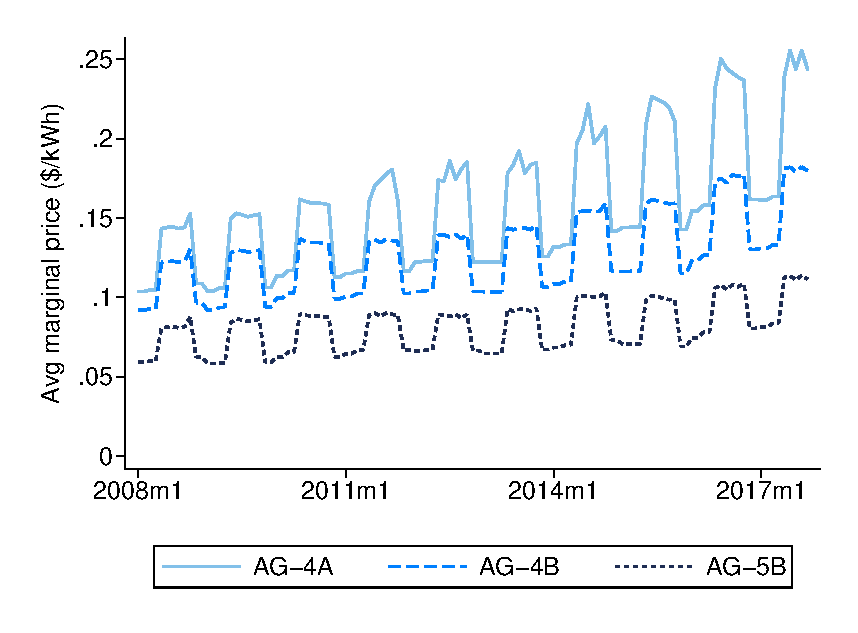
\includegraphics[width=.8\textwidth]{figures/marg_price_3rates.eps}}\\
\captionsetup{width=.85\textwidth}
\caption*{\footnotesize \emph{Notes:} This figure reports the times series of monthly average marginal electricity prices (\$/kWh) for three of the most common agricultural tariffs. Prices are systematically higher during summer months (May--October). Much of our identifying variation in monthly electricity prices comes from these monthly price times series not rising perfectly in parallel. }
\end{figure}


\begin{figure}[h!]\centering
\captionsetup{width=\textwidth}
\caption{PGE Agricultural Customers}
\label{fig:pge_ca_map}
\vspace{-2mm}
{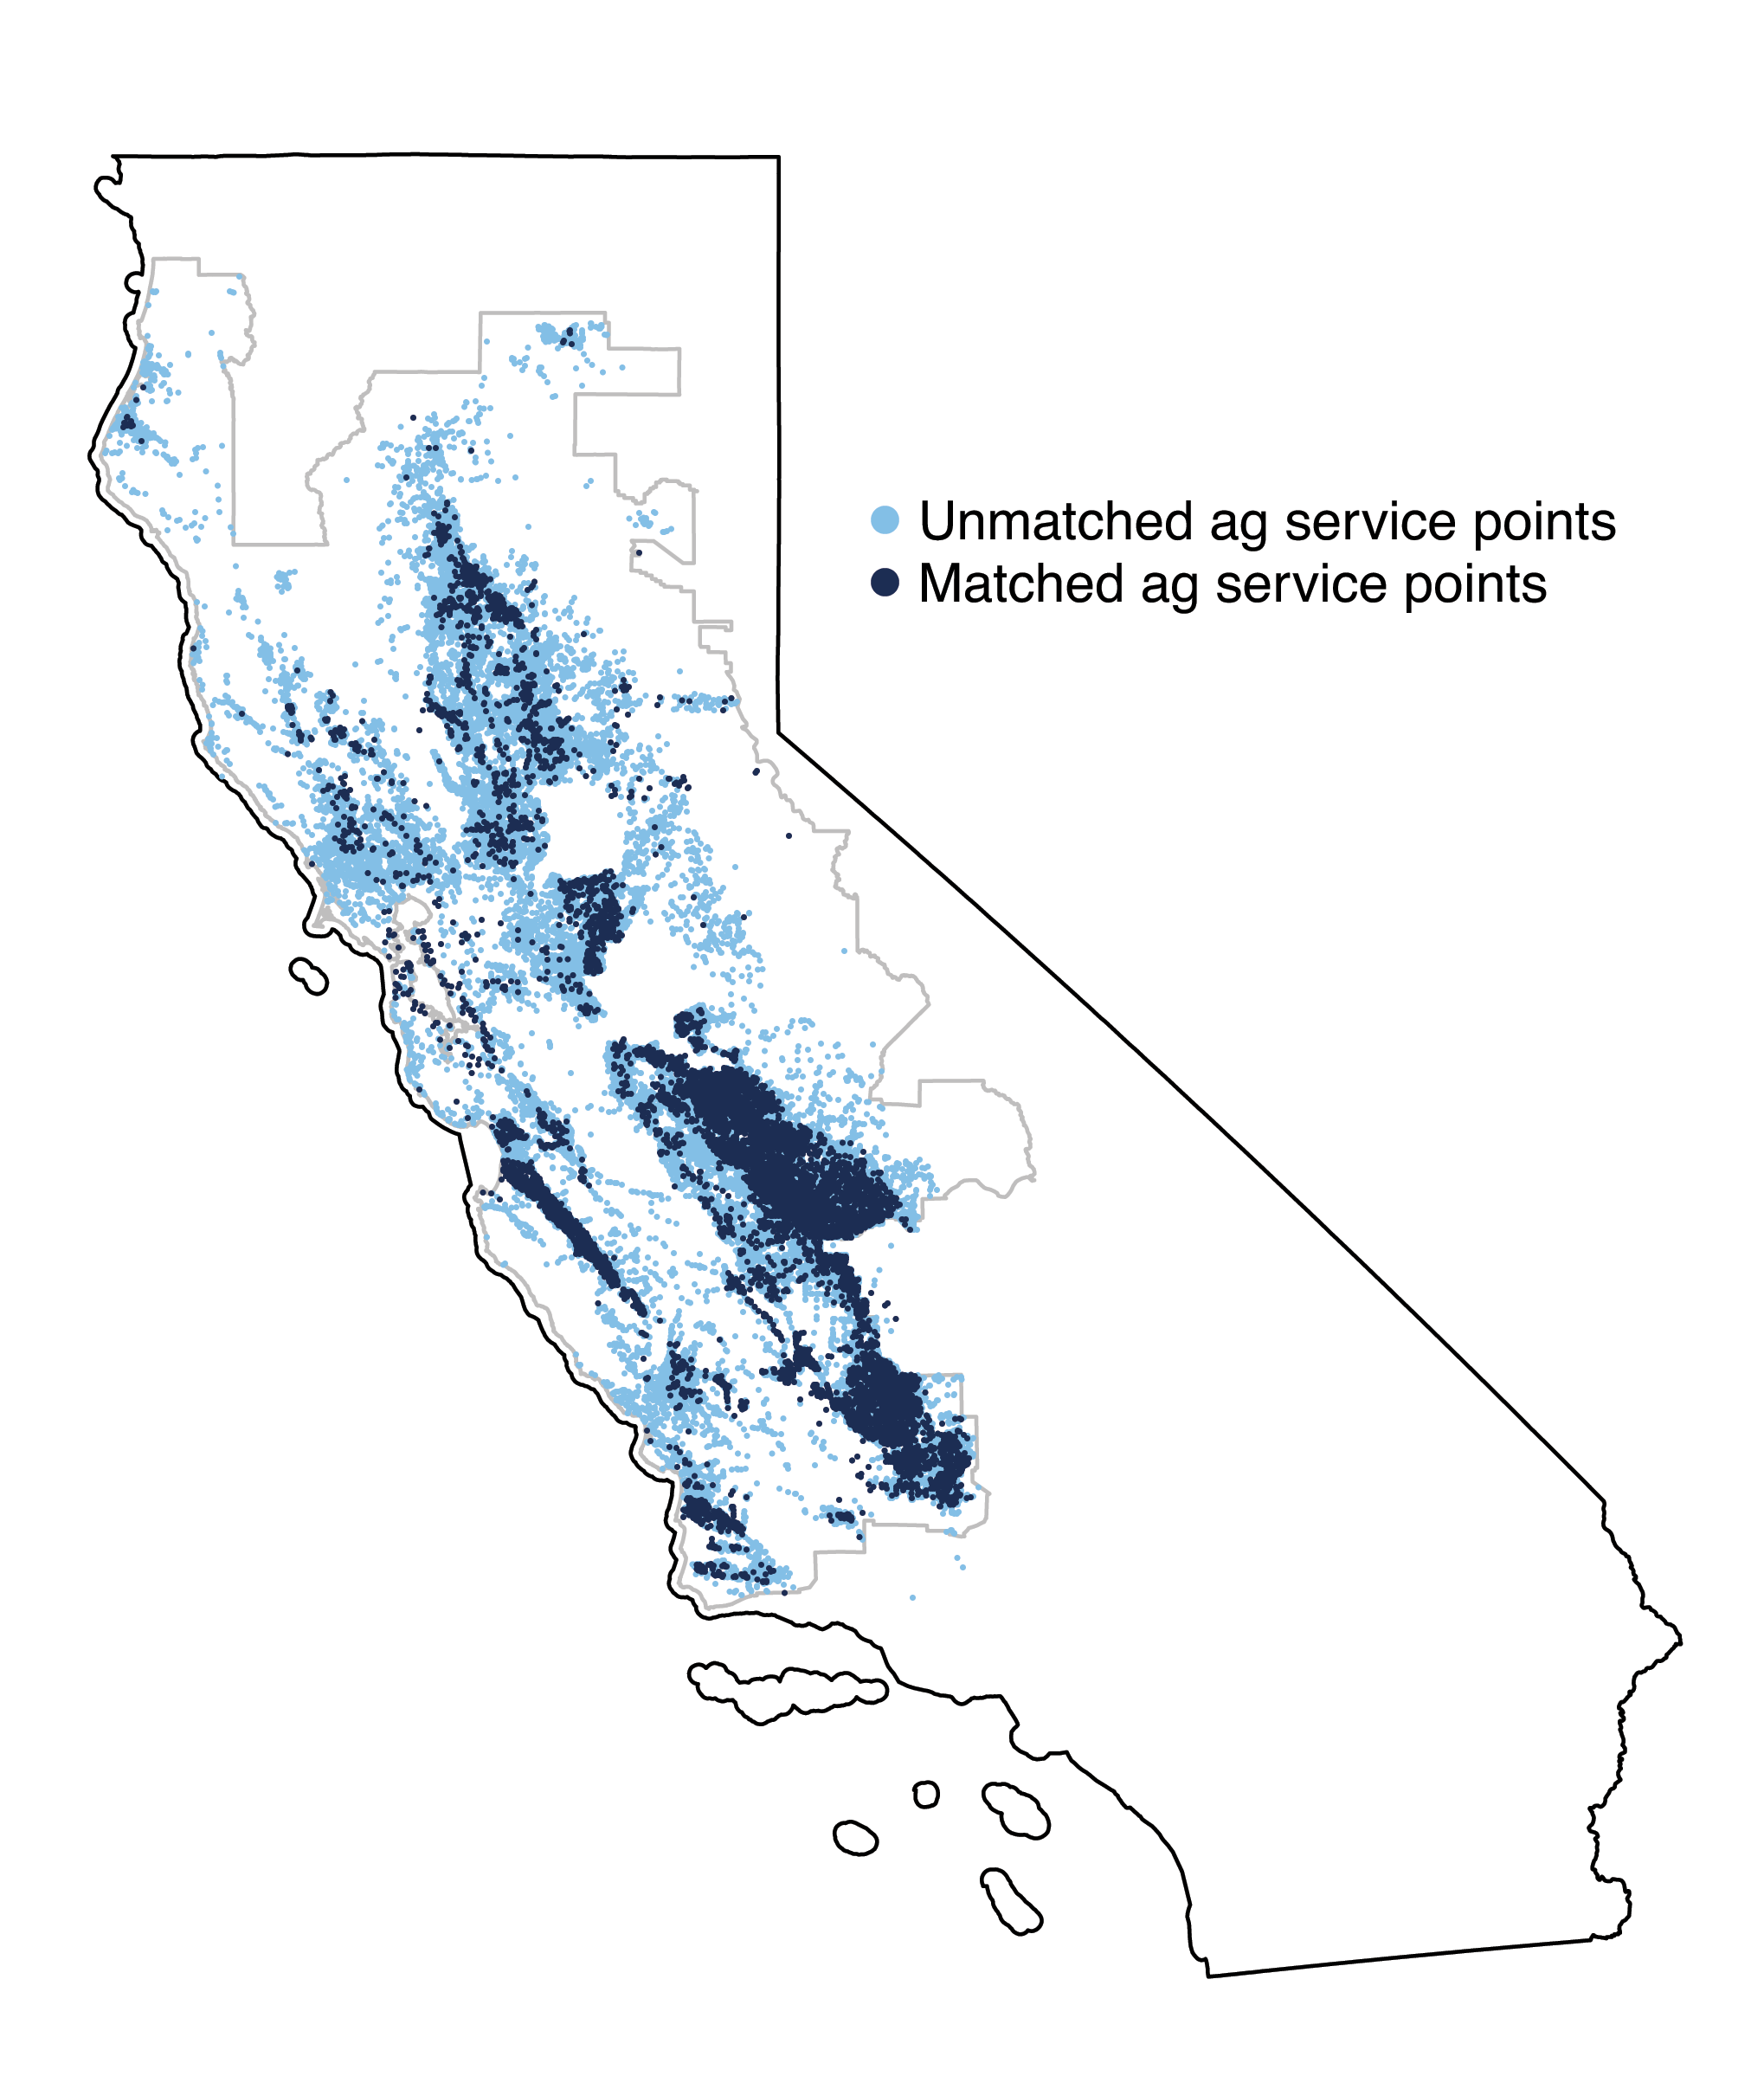
\includegraphics[width=.8\textwidth, trim={2mm 20mm 2mm 45mm}, clip]{figures/pge_ca_map.png}}\\
\captionsetup{width=.85\textwidth}
\caption*{\footnotesize \emph{Notes:} This figure maps the locations of all agricultural service points served by PGE. Dark blue dots indicate the 11,851 service point that we can match directly to an APEP pump test. Light blue dots indicate unmatched agricultural service points. The light grey outline is the geographic boundary of PGE's service territory. }
\end{figure}

\begin{figure}[t]
\begin{centering}
\caption{Histogram of pump horsepower}
\label{fig:pump_hist}
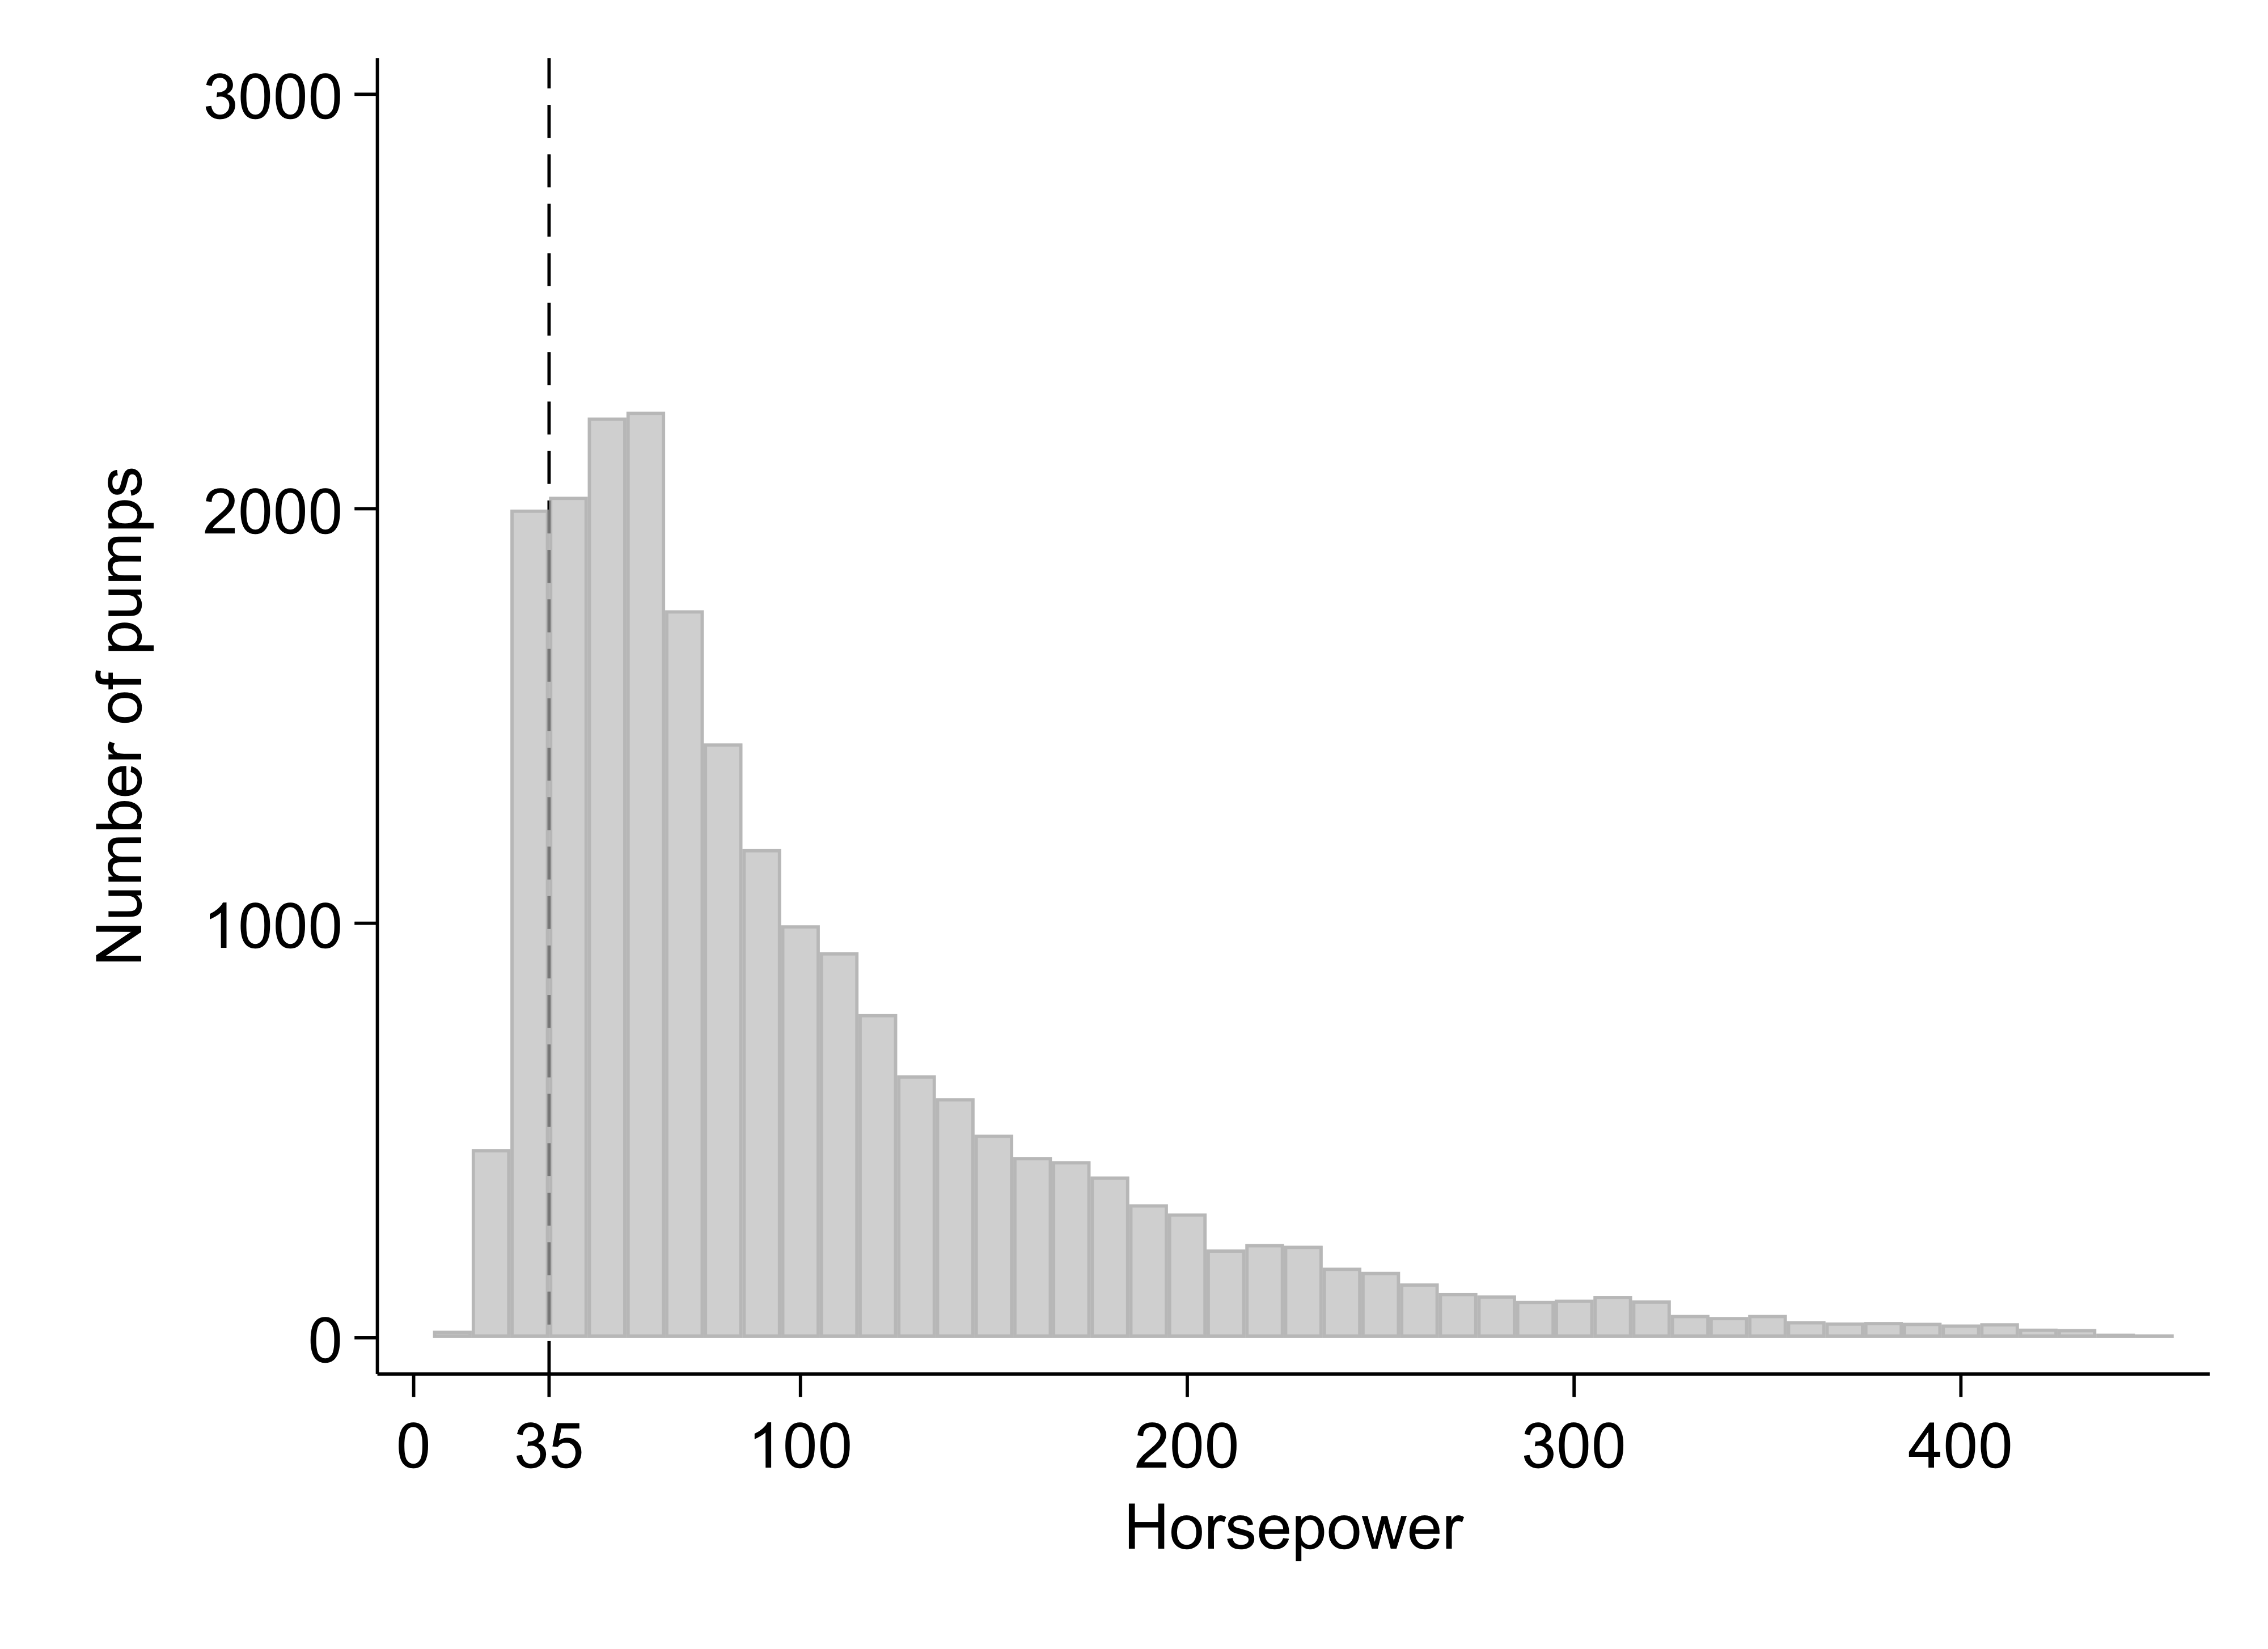
\includegraphics[width=0.7\textwidth]{Figures/pump_hist.png}
\caption*{\footnotesize \emph{Notes:} This is a histogram of measured horsepower for all 21,851 tests in our APEP pump test dataset. We observe no bunching on either side of the 35 hp cutoff that determines whether PGE classifies pumps as small or large. Bunching would be a sign that farmers optimize against PGE's tariff schedules when making pump investment decisions.}
\end{centering}
\end{figure}



\begin{figure}[t]
\begin{centering}
\caption{Modeling farm $i$'s water costs and groundwater demand response}
\label{fig:water_cost_cartoons}
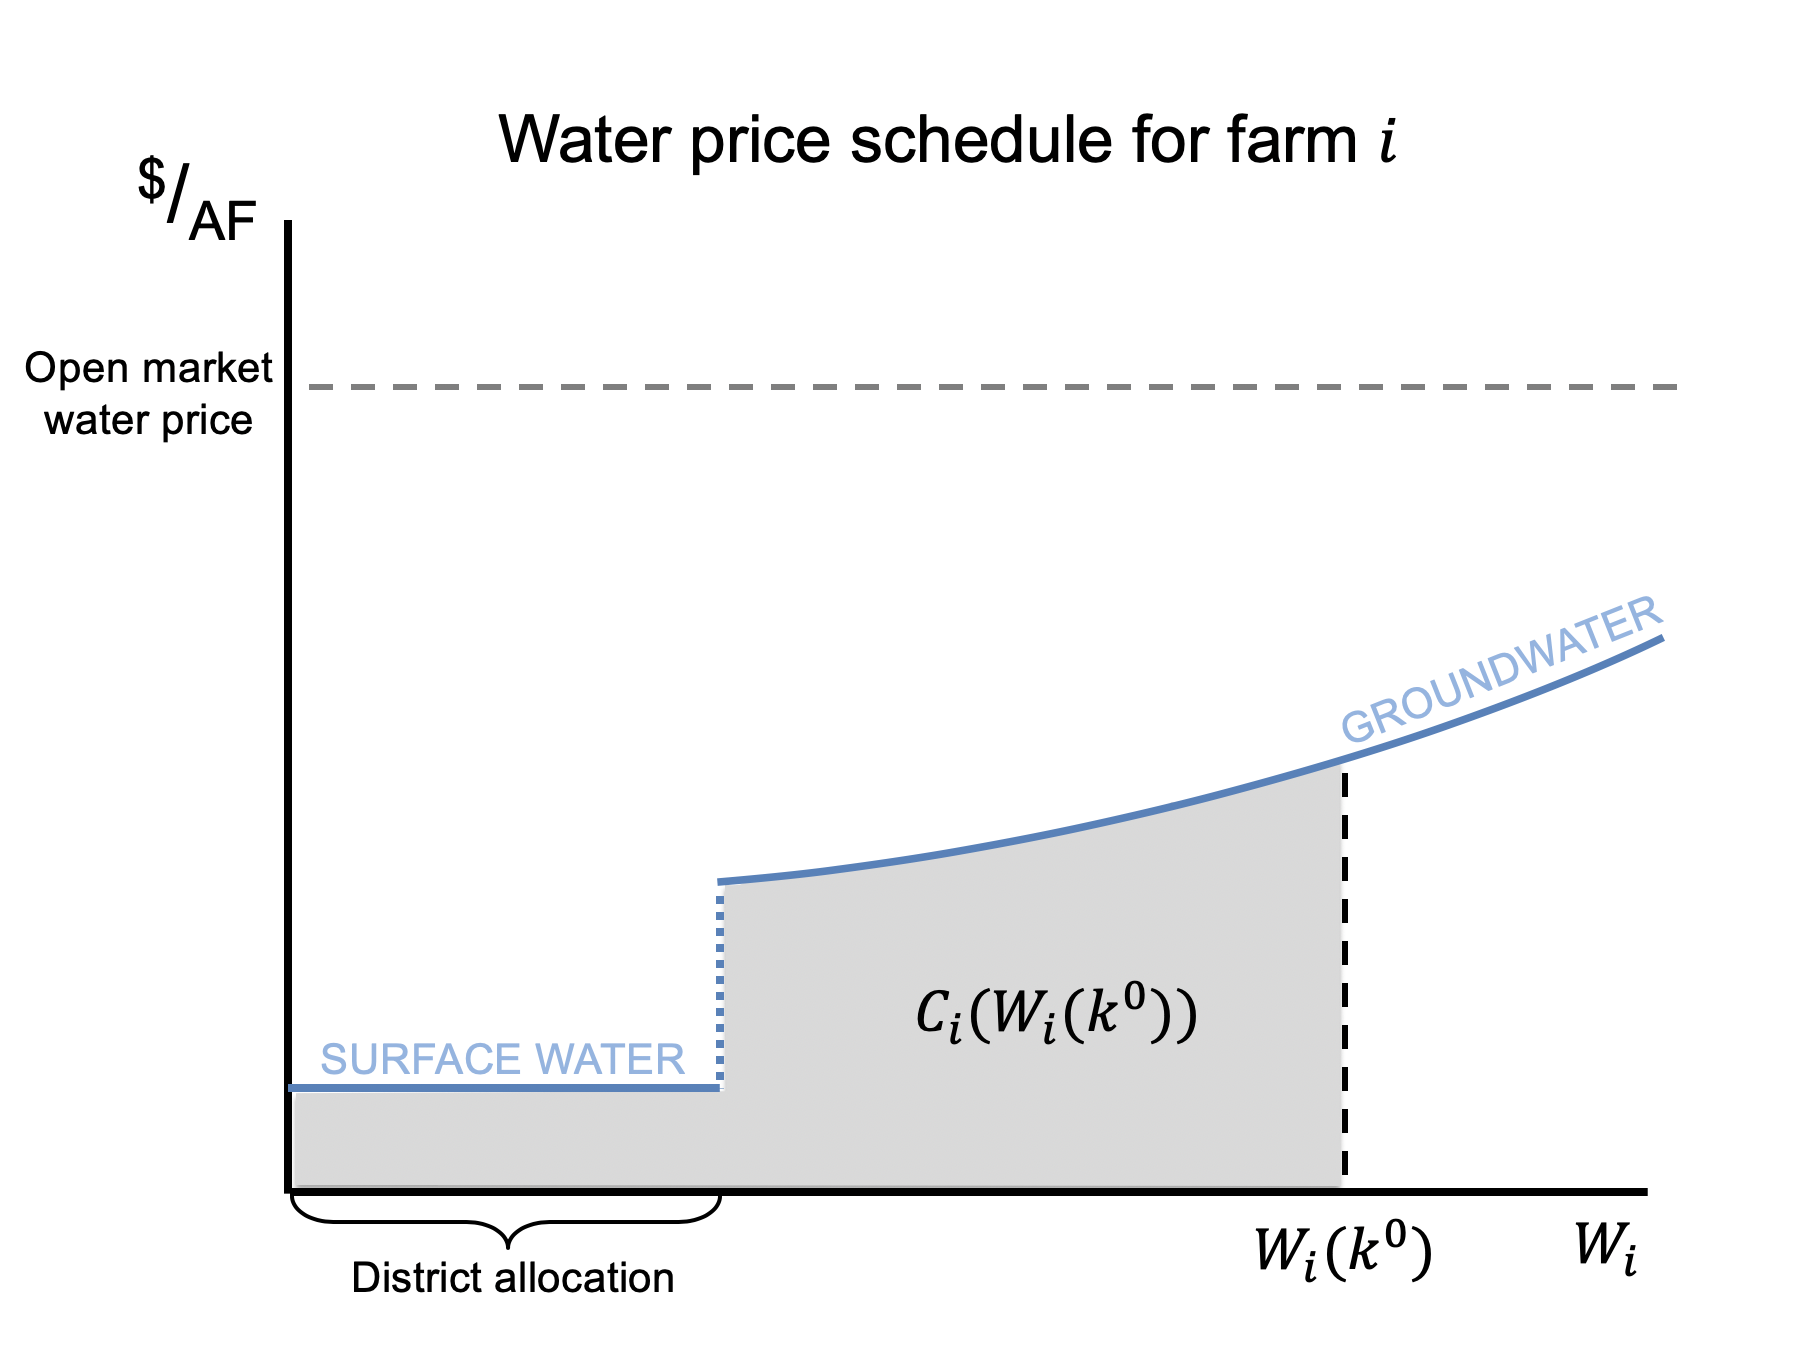
\includegraphics[width=0.495\textwidth, trim={4mm 0 11mm 0mm}, clip]{Figures/water_cost_1.png}
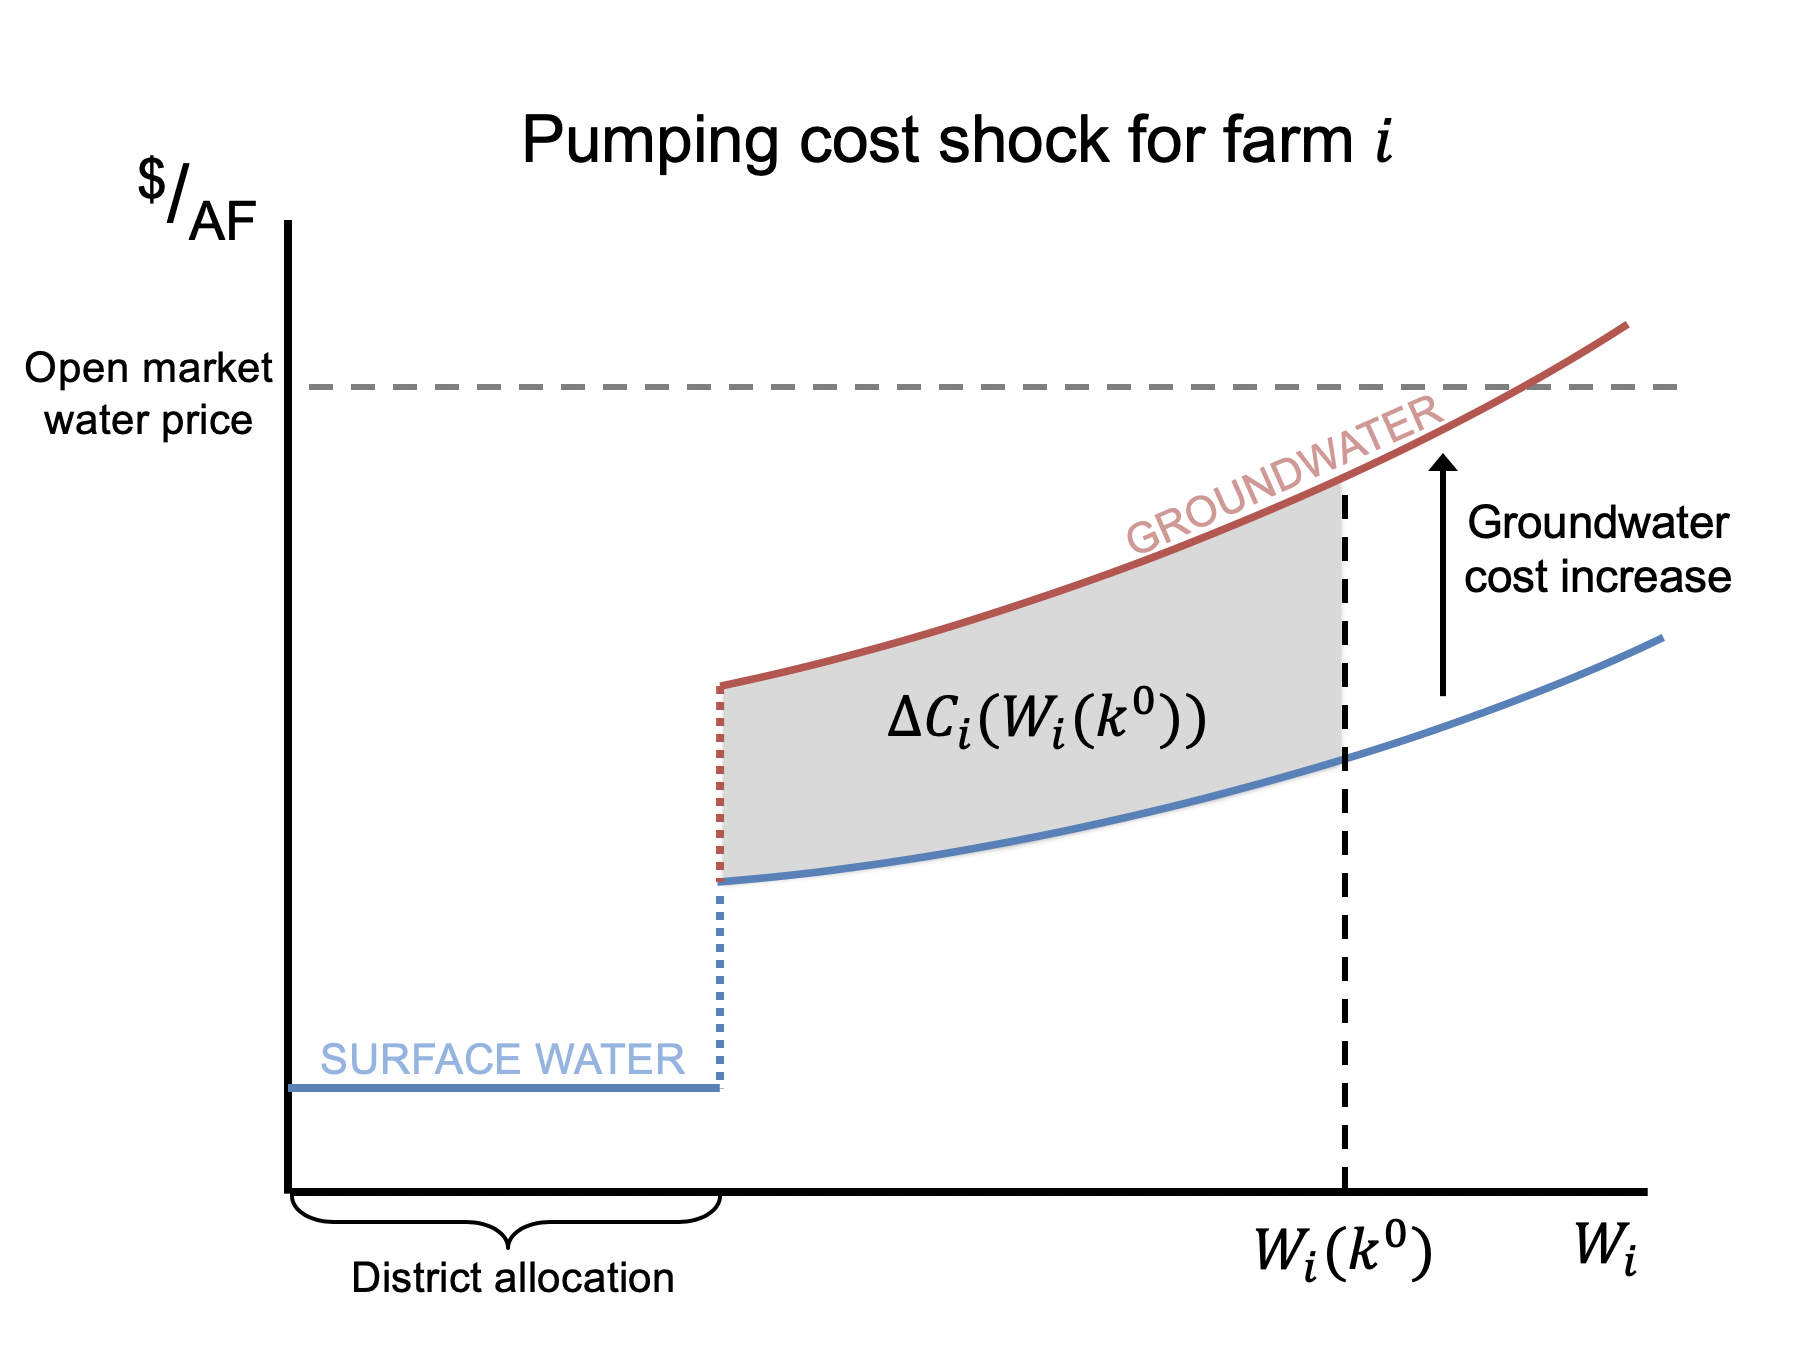
\includegraphics[width=0.495\textwidth, trim={4mm 0 11mm 0mm}, clip]{Figures/water_cost_2.png} \\
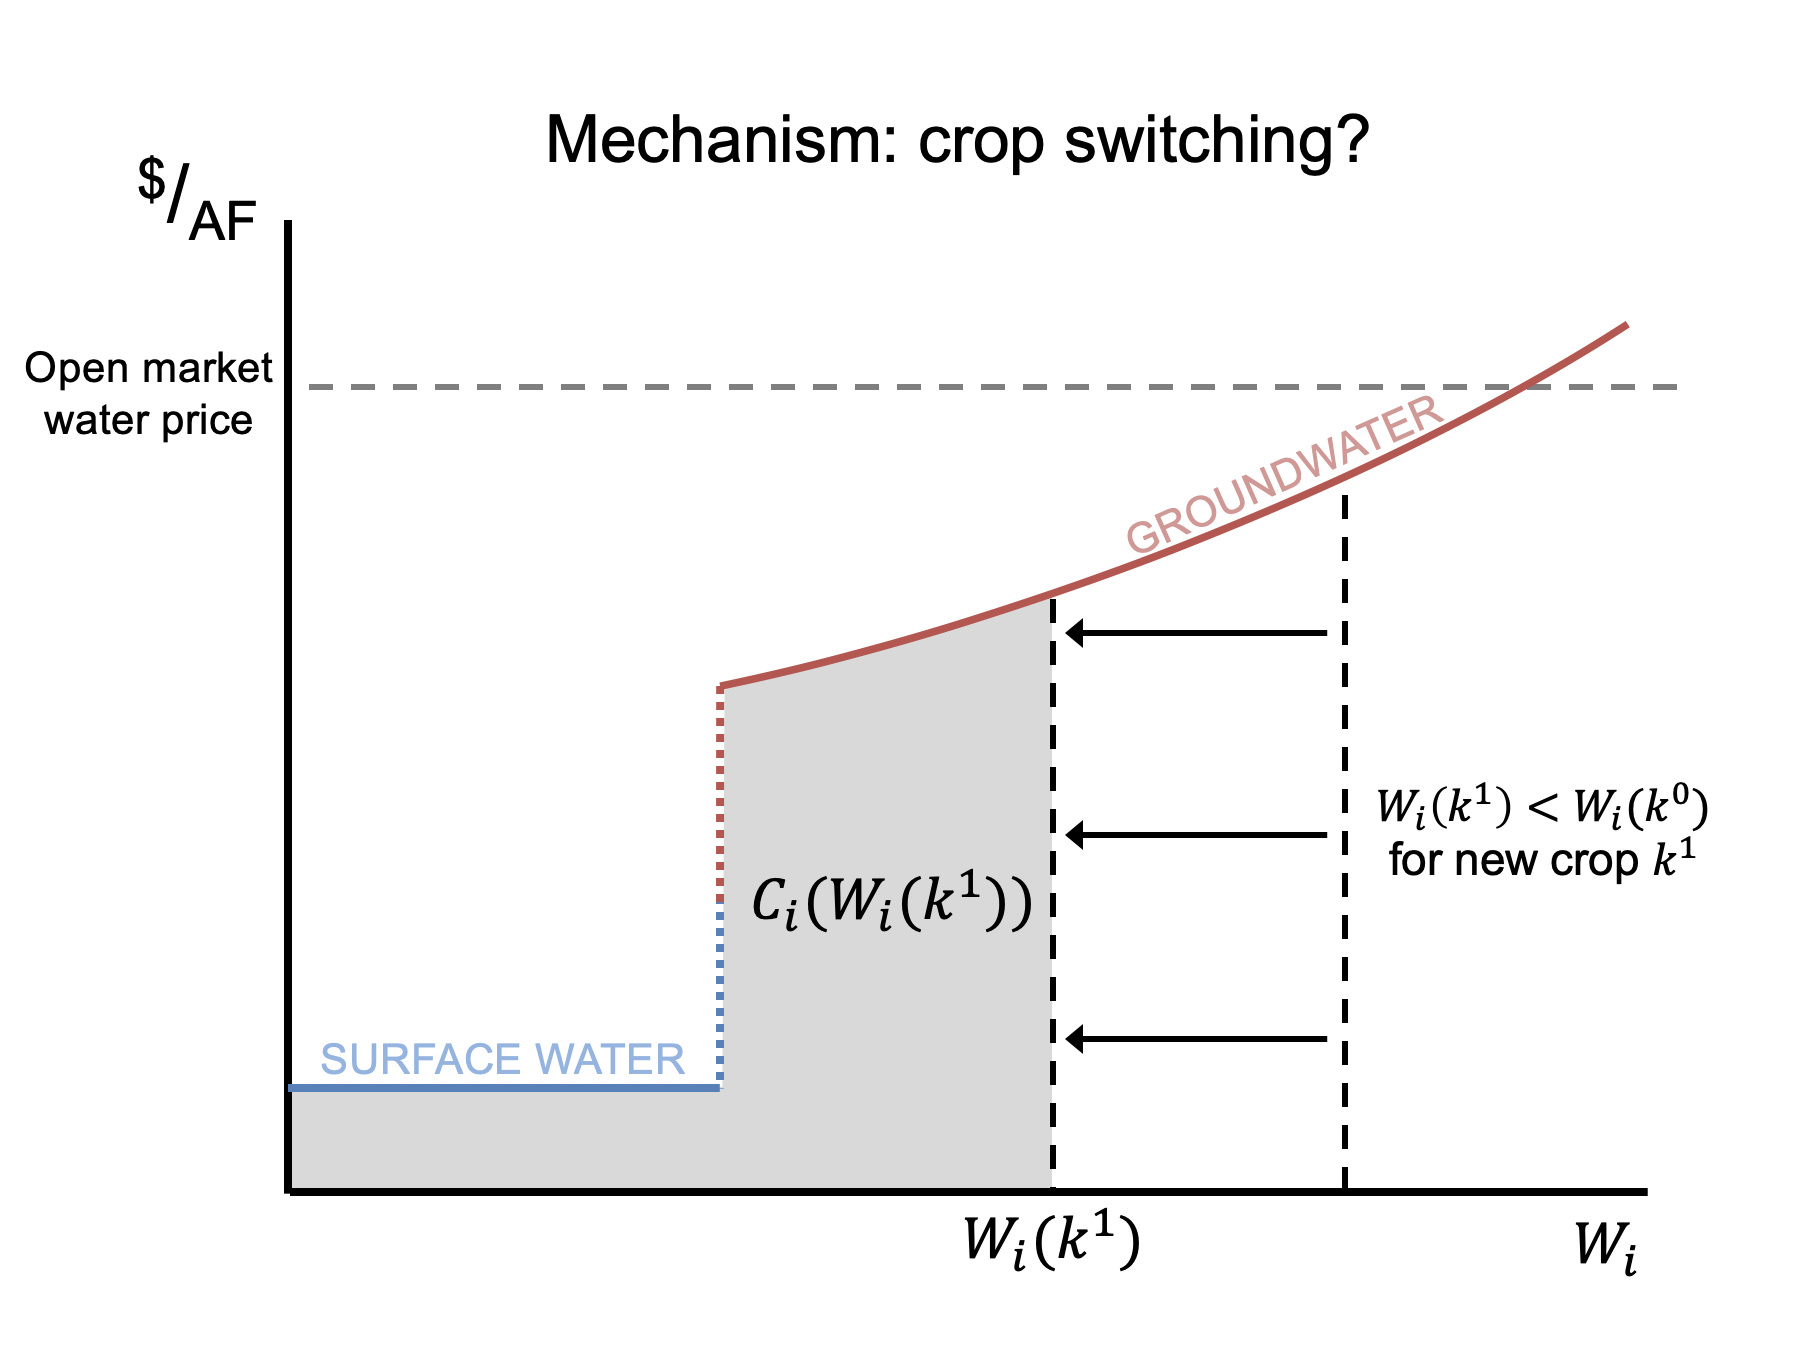
\includegraphics[width=0.495\textwidth, trim={4mm 0 11mm 0mm}, clip]{Figures/water_cost_3.png}
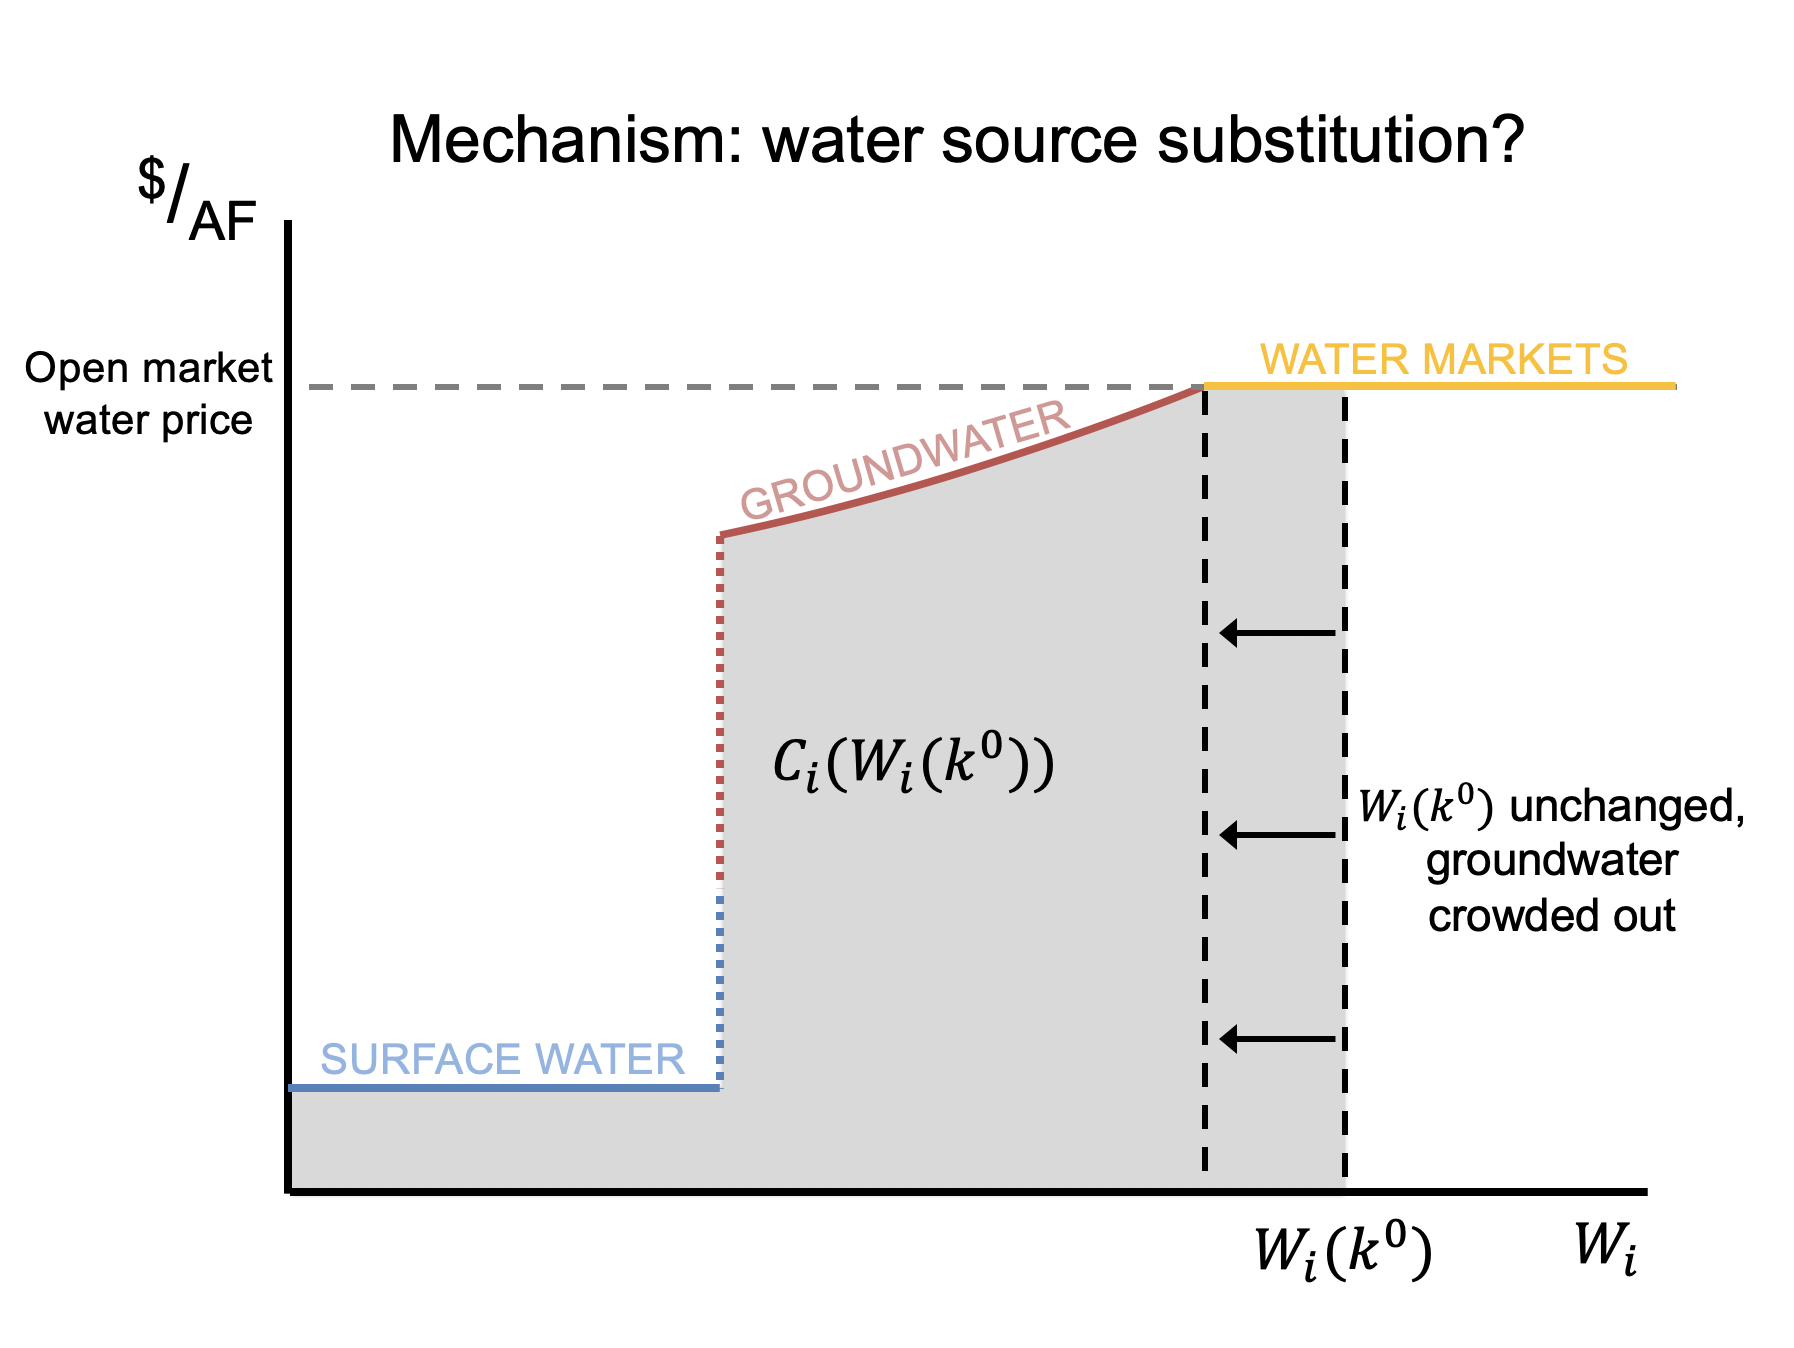
\includegraphics[width=0.495\textwidth, trim={4mm 0 11mm 0mm}, clip]{Figures/water_cost_4.png}
\caption*{\footnotesize \emph{Notes:} This figure presents a stylized water price schedule for a representative farm $i$. The price schedule is nonlinear and comprises water from up to three sources: (i) a low-cost allocation of surface water from farm $i$'s irrigation district; (ii) medium-cost groundwater pumping, with costs that rise gradually in own extraction; and (iii) a high-cost backstop of open market water transactions, for which we assume farm $i$ is a price taker. For crop $k^0$ requiring $W_i(k^0)$ acre/feet of water, farm $i$'s irrigation costs $C_i\big(W_i(k^0)\big)$ are represented by the shaded region in the top-left panel. If farm $i$ experiences a pumping cost shock (due to either an electricity price increase or a groundwater depth increase), its groundwater costs shift up and its total irrigation costs increase by the shaded region $\Delta C_i\big(W_i(k^0)\big)$ in the top-right panel. The bottom panels illustrate two ways that this pumping cost shock increase translate to a reduction in farm $i$'s groundwater consumption. First, the farmer may respond to this pumping cost shock by switching from crop $k^0$ to a less water intensive crop $k^1$, as in the bottom-left panel. Second, for a large enough cost shock, the farmer may continue to grow crop $k^0$, but substitute away from groundwater using open market water purchases.
}
\end{centering}
\end{figure}


\begin{figure}[t]
\begin{centering}
\caption{Profits in the Southern San Joaqu\'{i}n Valley Under Varying Water Prices}
\label{fig:davis_line_crossing}
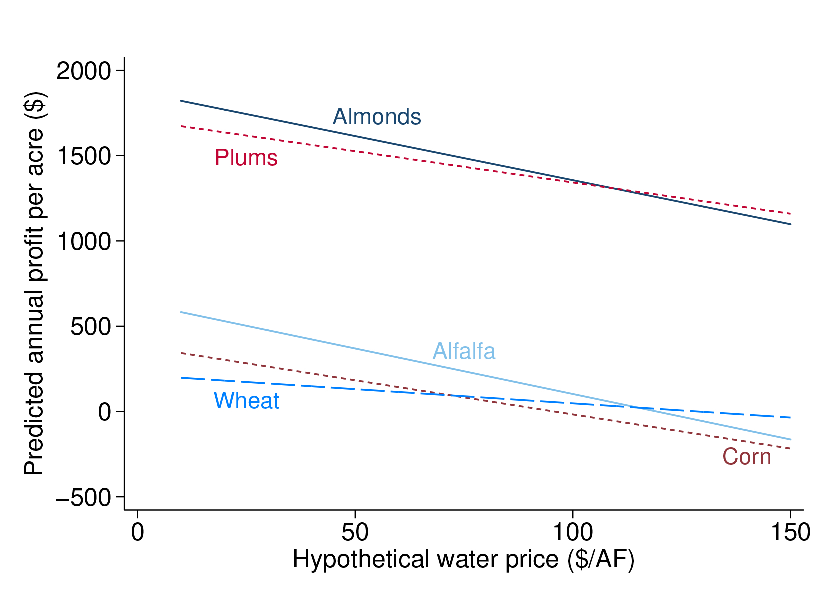
\includegraphics[width=0.7\textwidth]{Figures/davis_lines_crossing.pdf}
\caption*{\footnotesize \emph{Notes:} This figure plots annual profits per acre by crop, as reported by the UC Davis Cost Studies. We focus on five crop-specific studies in the Southern San Joaqu\'{i}n Valley, and vary the average cost of water for irrigation while holding all other assumptions constant.}
\end{centering}
\end{figure}


\begin{table}[b!]\centering
\footnotesize
\caption{PGE Agricultural Tariffs}
\label{tab:pge_ag_tariffs}
\vspace{-2mm}
\begin{adjustbox}{center}
\begin{tabular}{|c|c|c|c|}
\hline
\textbf{Category} & \textbf{Tariff} & \textbf{ Description} & \textbf{ Percent} \\
\hline
$ \begin{matrix}
\text{\bf Small pumps, conventional meters} \\
\text{single motor $<35$ hp, or} \\
\text{multiple motors summing to $<15$ hp}
\end{matrix} $
 & \textbf{1A} &  
\footnotesize $ \begin{matrix}
\text{High price per kWh (not time-varying),} \\
\text{fixed charge per hp connected} \\
\end{matrix} $ &  3.0 \\
\hline
$ \begin{matrix}
\text{\bf Large pumps, conventional meters} \\
\text{single motor $\ge 35$ hp, or} \\
\text{multiple motors summing to $\ge15$ hp,} \\
\text{or single overloaded motor $\ge 15$ hp}
\end{matrix} $ & \textbf{1B} &
\footnotesize $ \begin{matrix}
\text{High price per kWh (not time-varying),} \\
\text{fixed charge per max kW consumed} \\
\end{matrix} $ &  8.1 \\
\hline
\multirow{4}{*}{
$ \begin{matrix} \\ \\ \\ \\
\text{\bf Small pumps, smart meters} \\
\text{single motor $<35$ hp, or} \\
\text{multiple motors summing to $<15$ hp}
\end{matrix} $ 
} & \textbf{4A} (4D) & 
\footnotesize $ \begin{matrix}
\text{High prices per kWh (higher in peak hours),} \\
\text{fixed charges per hp connected, } \\
\text{very high peak prices on 14 summer Event Days} \\
\end{matrix} $ &  7.2 \\
\cline{2-4}
 & 5A (5D) &
\footnotesize $ \begin{matrix}
\text{Lower prices per kWh (peak \& offpeak),} \\
\text{no Event Day price increases, } \\
\text{higher fixed charges per hp} \\
\end{matrix} $ &  2.7 \\
\cline{2-4}
&  RA (RD) & 
\footnotesize $ \begin{matrix}
\text{Lower peak prices per kWh,} \\
\text{higher off-peak prices per kWh,} \\
\text{no Event Day price increases, } \\
\text{choice between MTW or WTF peak days} \\
\end{matrix} $ &  1.2 \\
\cline{2-4}
& VA (VD) & 
\footnotesize $ \begin{matrix}
\text{Lower peak prices per kWh,} \\
\text{higher off-peak prices per kWh,} \\
\text{no Event Day price increases, } \\
\text{choice of 3 shorter 4-hour peak periods} \\
\end{matrix} $ &  0.9 \\
\hline
\multirow{6}{*}{
$ \begin{matrix} \\ \\ \\ \\ \\ \\
\text{\bf Large pumps, smart meters} \\
\text{single motor $\ge 35$ hp, or} \\
\text{multiple motors summing to $\ge15$ hp,} \\
\text{or single overloaded motor $\ge 15$ hp}
\end{matrix} $
} & \textbf{4B}  (4E) & 
\footnotesize $ \begin{matrix}
\text{High prices per kWh (higher in peak hours),} \\
\text{fixed charges per max kW consumed} \\
\end{matrix} $ &  20.1 \\
\cline{2-4}
&  5B (5E) & 
\footnotesize $ \begin{matrix}
\text{Much lower prices per kWh (peak \& offpeak),} \\
\text{higher fixed charge per max kW} \\
\end{matrix} $ &  37.8 \\
\cline{2-4}
 & 4C (4F) &
\footnotesize $ \begin{matrix}
\text{Slightly lower prices per kWh (peak \& offpeak),} \\
\text{higher fixed charges per kW shifted to peak,} \\
\text{very high peak prices on 14 summer Event Days} \\
\end{matrix} $ &  2.4 \\
\cline{2-4}
& 5C (5F) &
\footnotesize $ \begin{matrix}
\text{Much lower prices per kWh (peak \& offpeak),} \\
\text{higher fixed charges per kW shifted to peak,} \\
\text{very high peak prices on 14 summer Event Days} \\
\end{matrix} $ &  7.8 \\
\cline{2-4}
& RB (RE) & 
\footnotesize $ \begin{matrix}
\text{Higher prices per kWh (peak \& off-peak),} \\
\text{choice between MTW or WTF peak days,} \\
\text{lower fixed charges per max kW (in summer)} \\
\end{matrix} $ &  1.5 \\
\cline{2-4}
& VB (VF) & 
\footnotesize $ \begin{matrix}
\text{Higher prices per kWh (peak \& off-peak),} \\
\text{choice of 3 shorter 4-hour peak periods,} \\
\text{lower fixed charges per max kW (in summer)} \\
\end{matrix} $ &  0.6 \\
\hline
$ \begin{matrix}
\text{\bf Customers transitioning off} \\
\text{\bf internal combustion engines}
\end{matrix} $
 & \textbf{ICE} & 
\footnotesize $ \begin{matrix}
\text{Very low price per kWh (high in peak hours),} \\
\text{fixed charge per max kW consumed} \\
\end{matrix} $ & 6.8 \\
\hline
\end{tabular}
\end{adjustbox}
 \captionsetup{width=1.1\textwidth}
\caption*{\scriptsize \emph{Notes:}
This table provides a rough summary of PGE's 23 electricity tariffs for agricultural customers. 
The first column lists the 5 disjoint categories of customers, defined (primarily) by physical pumping capital and electricity meters.
Effective default tarrifs within each group are in bold, and farmers may switch tariffs \emph{within} a category (but not \emph{across} categories).
All tariffs have fixed (\$/kW) and volumetric (\$/kWh) prices that vary by summer vs.\ winter. 
All time-of-use tariffs (i.e. all but 1A and 1B) also vary between peak (12:00pm--6:00pm on summer weekdays), partial peak (8:30am--9:30pm on weekends), and off-peak periods.
DEF tariffs are functionally equivalent to their ABC analogs, and are holdovers for the earliest customers to adopt time-of-use pricing.
Actual tariffs are far more complex, and tariff documents are available at \url{https://www.pge.com/tariffs/index.page}.
The right-most column reports the percent of observations in our main estimation sample on each tariff.
}
\end{table}

\begin{table}\centering
\caption{\normalsize Summary Statistics -- Electricity Data}
\label{tab:elec_summary_stats}
\begin{tabular}{lrcrcrr}
\hline
\hline
\\ 
\vspace{-8mm}
\\
&& $\begin{matrix}\text{All Ag}\\ \text{Customers}\end{matrix}$  && $\begin{matrix}\text{Matched} \\ \text{to Pumps}\end{matrix}$ \\
[.1em]
\cline{3-5}
\\
\vspace{-7mm}
\\
Service point-month observations && 9,991,458 && 1,168,553 \\ 
[.2em]
Unique service points (SPs) && 108,172 && 11,851 \\ 
[.2em]
SPs that switch tariff categories  && 44,414 && 2,844   \\
[.2em]
SPs that switch categories (pumping capital)  && 3,454 && 561   \\
[.2em]
SPs that switch categories (smart meters)  && 43,045 && 2,553   \\
[.2em]
Share of SP-months on time-varying tariffs  && 0.702 && 0.886   \\
[.2em]
Share of SP-months on peak-day tariffs  && 0.295 && 0.152   \\
[1.4em]
Monthly electricity consumption (kWh) && 6080.9 && 12055.7   \\
 && (39783.1) && (25075.1)   \\
[.4em]
Monthly electricity consumption (kWh), summer && 8249.6 && 17589.1   \\
 && (45660.8) && (29818.5)   \\
[.4em]
Monthly electricity consumption (kWh), winter && 3849.7 && 6362.8   \\
 && (32498.8) && (17232.5)   \\
[1.4em]
Average marginal electricity price (\$/kWh) && 0.148 && 0.113   \\
 && (0.050) && (0.042)   \\
[.4em]
Average marginal electricity price (\$/kWh), summer && 0.171 && 0.130   \\
 && (0.051) && (0.044)   \\
[.4em]
Average marginal electricity price (\$/kWh), winter && 0.126 && 0.096   \\
 && (0.037) && (0.032)   \\
[1.4em]
Average monthly bill (\$, non-zero bills) && 936.66 && 1814.15   \\
 && (4662.71) && (3285.26)   \\
[.4em]
Average monthly bill (\$, non-zero bills), summer && 1398.90 && 2821.16   \\
 && (5847.34) && (4020.99)   \\
[.4em]
Average monthly bill (\$, non-zero bills), winter && 456.17 && 764.99   \\
 && (2888.86) && (1742.21)   \\
[.2em]
\hline
\end{tabular}
\captionsetup{width=\textwidth}
\caption*{\scriptsize \emph{Notes:} The left column reports summary statistics 
for the universe of agricultural electricity customers in PGE service territory, from 2008--2017.
The right column includes the subset of agricultural customers that we successfully match to a 
groundwater pump in the APEP pump test dataset---i.e., our main estimation sample.
``Pumping capital'' denotes tariff category switches driven by shifts between small pumps ($<35$ hp) and 
large pumps ($\ge 35$ hp), or adding/removing an auxiliary internal combustion engine.
Most tariff category switches were driven by PGE's smart meter rollout.
Time-varying tariffs (i.e.\ all except 1A and 1B) have higher marginal prices during peak demand hours. 
Peak-day tariffs (i.e.\ 4A, 4D, 4C, 4F, 5C, 5F) have very high marginal prices during peak
hours on the 14 highest-demand summer days.
Monthly bills include both volumetric (\$/kWh) and fixed charges (\$/kW, \$/hp, and \$/day).
Summer months are May--October.
Standard deviations of sample means in parentheses.
}
\end{table}


\begin{table}\centering
\caption{\normalsize Summary statistics -- Pump tests and groundwater consumption}
\label{tab:water_summary_stats}
\begin{tabular}{lrcrcrr}
\hline
\hline
\\ 
\vspace{-8mm}
\\
&& $\begin{matrix}\text{Matched to Pumps}\end{matrix}$ \\
[.1em]
\cline{2-3}
\\
\vspace{-7mm}
\\
Service point-month observations && 1,168,511 \\ 
[.2em]
Unique service points (SPs) && 11,849 \\ 
[1.4em]
Matched APEP points per SP && 1.67 \\ 
 && (1.73) \\
[.4em]
Operating pump efficiency (\%) && 54.46   \\
 && (11.52)   \\
[.4em]
kWh per AF conversion factor (APEP measured) && 430.35   \\
 && (254.23)   \\
[.4em]
kWh per AF conversion factor (constructed) && 321.12   \\
 && (185.81)   \\
[1.4em]
Monthly groundwater consumption (AF) && 46.8   \\
 && (133.1)   \\
[.4em]
Monthly groundwater consumption (AF), summer && 69.7   \\
 && (155.8)   \\
[.4em]
Monthly groundwater consumption (AF), winter && 23.2   \\
 && (99.4)   \\
[1.4em]
Average marginal groundwater price (\$/AF) && 40.35   \\
 && (30.08)   \\
[.4em]
Average marginal groundwater price (\$/AF), summer && 43.27   \\
 && (32.38)   \\
[.4em]
Average marginal groundwater price (\$/AF), winter && 37.34   \\
 && (27.19)   \\
[.2em]
\hline
\vspace{-2mm}
\end{tabular}
\captionsetup{width=.93\textwidth}
\caption*{\scriptsize \emph{Notes:} These summary stats are from the merged panel of 
groundwater prices and quantities, which combines electricity data, pump test data, and groundwater data.
We observe 3.45 unique APEP pump tests for the average matched service point, although 37 percent of 
service points match to only a single APEP test.
Our constructed kWh per AF conversion factor (i.e. $\widehat{\text{kWh}\big/\text{AF}}_{it}$) uses monthly 
groundwater rasters to capture changes in (measured) kWh per AF over time, and estimation error 
compresses the right tail of distribution of measured kWh per AF. 
Monthly groundwater consumption divides electricity consumption (kWh) by $\widehat{\text{kWh}\big/\text{AF}}_{it}$. 
Grounwater prices multiply marignal electricity prices (\$/kWh) by $\widehat{\text{kWh}\big/\text{AF}}_{it}$. 
Summer months are May--October.
Standard deviations of sample means in parentheses.
}
\end{table}


\begin{table}[t!]\centering
\small
\caption{Estimated Demand Elasticities -- Electricity  \label{tab:elec_regs_main}}
\vspace{-0.1cm}
\small
\begin{adjustbox}{center} 
\begin{tabular}{lcccccccc} 
\hline \hline
\vspace{-0.37cm}
\\
 & (1)  & (2)  & (3)  & (4)  & (5)  & (6) \\ 
[0.1em]
 & OLS & IV & IV & IV & IV & IV \\
\vspace{-0.37cm}
\\
\cline{2-7}
\vspace{-0.27cm}
\\
 $\log\big(P^{\text{elec}}_{it}\big)$ ~ & $-1.31$$^{***}$  & $-1.58$$^{***}$ & $-1.17$$^{***}$ & $-1.02$$^{***}$ & $-1.18$$^{***}$  & $-0.76$$^{***}$ \\ 
& $(0.11)$ & $(0.17)$ & $(0.16)$ & $(0.14)$ & $(0.21)$ & $(0.17)$ \\
[1.5em] 
Instrument(s): \\
[0.1em] 
~~ Default $\log\big(P^{\text{elec}}_{it}\big)$  & & Yes & Yes  & Yes  & & Yes \\
[0.1em] 
~~ Default $\log\big(P^{\text{elec}}_{it}\big)$, lagged  & & & & & Yes & \\
[1.5em] 
Fixed effects: \\
[0.1em] 
~~Unit $\times$ month-of-year  & Yes  & Yes  & Yes  & Yes  & Yes  & Yes   \\ 
[0.1em] 
~~Month-of-sample  & Yes  & Yes  & Yes  & Yes  & Yes  & Yes   \\ 
[0.1em] 
~~Unit $\times$ physical capital & & & Yes & Yes & Yes & Yes  \\
[0.1em] 
~~Water basin $\times$ year & & &  & Yes &  &   \\
[0.1em] 
~~Water district $\times$ year & & &  & Yes &  &  \\
[0.1em] 
~~Unit-specific linear time trends & & & & & &  Yes \\
[1.5em] 
Service point units & 11,175 & 11,175 & 11,175 & 11,121 & 10,924 & 11,175  \\ 
[0.1em] 
Months  & 117 & 117 & 117 & 117 & 105 & 117 \\ 
[0.1em] 
Observations & 1.05M & 1.05M & 1.05M & 1.04M & 0.91M & 1.05M \\ 
[0.1em] 
First stage $F$-statistic &  & 4136 & 7382 & 7508 & 757 & 4776 \\ 
[0.15em]
\hline
\end{tabular}
\end{adjustbox}
\captionsetup{width=\textwidth}
\caption*{\scriptsize \emph{Notes:} Each regression estimates Equation (\ref{eq:reg_elec}) at the service point by month level,
where the dependent variable is the inverse hyperbolic sine transformation of electricity consumed by service point $i$ in month $t$.
We estimate IV specifications via two-stage least squares, instrumenting with either unit $i$'s within-category default 
logged electricity price in month $t$ \emph{or} the 6- and 12- month lags of this variable.
``Physical capital'' is a categorical variable for (i) small pumps, (ii) large pumps, and (iii) internal combustion engines, and unit $\times$
physical capital fixed effects control for shifts in tariff category triggered by the installation of new pumping equipment.
Water basin $\times$ year fixed effects control for broad geographic trends in groundwater depth.
Water district $\times$ year fixed effects control for annual variation in surface water allocations.
All regressions drop solar NEM customers, customers with bad geocodes, and months with irregular electricity bills
(e.g.\ first/last bills, bills longer/shorter than 1 month, overlapping bills for a single account).
Standard errors (in parentheses) are clustered by service point and by month-of-sample.
Significance: *** $p < 0.01$, ** $p < 0.05$, * $p < 0.10$.
}
\end{table}


\begin{table}[t!]\centering
\small
\caption{Estimated Demand Elasticities -- Groundwater  \label{tab:water_regs_main}}
\vspace{-0.1cm}
\small
\begin{adjustbox}{center} 
\begin{tabular}{lcccccccc} 
\hline \hline
\vspace{-0.37cm}
\\
 & (1)  & (2)  & (3)  & (4)  & (5)  & (6) \\ 
[0.1em]
 & IV & IV & IV & IV & IV & IV \\
\vspace{-0.37cm}
\\
\cline{2-7}
\vspace{-0.27cm}
\\
 $\log\big(P^{\text{elec}}_{it}\big)$: $\hat\beta^{\text{e}}$ ~ & 
 $-1.21$$^{***}$  & $-1.39$$^{***}$ & $-1.38$$^{***}$ & $-1.26$$^{***}$ & $-1.23$$^{***}$  & $-1.68$$^{***}$ \\ 
& $(0.17)$ & $(0.18)$ & $(0.19)$ & $(0.17)$ & $(0.16)$ & $(0.21)$ \\
[0.75em] 
 $\log\Big(\widehat{\tfrac{{\text{kWh}}}{\text{AF}}}_{it}\Big)$: $\hat\beta^{\text{w}}$ ~ & 
 $-0.92$$^{***}$  & $-1.37$$^{***}$ & $-1.32$$^{***}$ & $-1.72$$^{***}$ & $-1.24$$^{***}$  & $-2.04$$^{***}$ \\ 
[-0.3em] 
& $(0.11)$ & $(0.25)$ & $(0.28)$ & $(0.30)$ & $(0.24)$ & $(0.45)$ \\
[1.5em] 
Instrument(s): \\
[0.1em] 
~~ Default $\log\big(P^{\text{elec}}_{it}\big)$  & Yes & Yes & Yes  & Yes  & Yes & Yes \\
[0.1em] 
~~ $\log\big(\text{Avg depth in basin}\big)$  & & Yes & Yes & Yes & Yes & \\
[0.1em] 
~~ $\log\big(\text{Avg depth in basin}\big)$, lagged  & & & & & & Yes \\
[1.5em] 
Fixed effects: \\
[0.1em] 
~~Unit $\times$ month-of-year  & Yes  & Yes  & Yes  & Yes  & Yes  & Yes   \\ 
[0.1em] 
~~Month-of-sample  & Yes  & Yes  & Yes  & Yes  & Yes  & Yes   \\ 
[0.1em] 
~~Unit $\times$ physical capital & Yes & Yes & Yes & Yes & Yes & Yes  \\
[0.1em] 
~~Water basin $\times$ year & & &  & & Yes &   \\
[0.1em] 
~~Water district $\times$ year & & & & & Yes &  \\
[1.5em] 
Groundwater time step & Month & Month & Month & Quarter & Month & Month  \\ 
[0.1em] 
Only basins with $>1000$ SPs &  &  & Yes &  &  &   \\ 
[1.5em] 
Service point units & 10,159 & 10,121 & 9,324 & 10,134 & 10,086 & 9,890  \\ 
[0.1em] 
Months  & 117 & 116 & 116 & 117 & 116 & 105 \\ 
[0.1em] 
Observations & 0.93M & 0.83M & 0.80M & 0.89M & 0.83M & 0.70M \\ 
[0.1em] 
First stage $F$-statistic & 6932 & 129 & 144 & 61 & 69 & 20 \\ 
[0.15em]
\hline
\end{tabular}
\end{adjustbox}
\captionsetup{width=\textwidth}
\caption*{\scriptsize \emph{Notes:} 
Each regression estimates Equation (\ref{eq:reg_water}) at the service point by month level,
where the dependent variable is the inverse hyperbolic sine transformation 
of electricity consumed by service point $i$ in month $t$.
We report estimates for $\hat\beta^{\text{e}}$ and $\hat\beta^{\text{w}}$, where the latter subtracts 
1 from the estimated coefficient on $\log \big(\widehat{\text{kWh}\big/\text{AF}}_{it}\big)$.
We estimate IV specifications via two-stage least squares, and all regressions instrument 
for $P^{\text{elec}}_{it}$ with unit $i$'s within-category default logged electricity price 
in month $t$ (consistent with our preferred specification from Table \ref{tab:elec_regs_main}).
We instrument for $\log \big(\widehat{\text{kWh}\big/\text{AF}}_{it}\big)$ with either logged 
average groundwater depth across unit $i$'s basin, or the 6- and 12-month lags of this variable.
``Physical capital'' is a categorical variable for (i) small pumps, (ii) large pumps, and (iii) 
internal combustion engines, and unit $\times$ physical capital fixed effects control for shifts 
in tariff category triggered by the installation of new pumping equipment.
Water basin $\times$ year fixed effects control for broad geographic trends in groundwater depth.
Water district $\times$ year fixed effects control for annual variation in surface water allocations.
Column (3) restricts the sample to only the three most common water basins (San Joaquin Valley, 
Sacramento Valley, and Salinas Valley), each of which contains over 1000 unique SPs in our estimation sample.
Column (4) uses a quarterly panel of groundwater depths to construct $\log \big(\widehat{\text{kWh}\big/\text{AF}}_{it}\big)$ 
and the instrument, rather than a monthly panel.
All regressions drop solar NEM customers, customers with bad geocodes, months with irregular electricity bills 
(e.g.\ first/last bills, bills longer/shorter than 1 month, overlapping bills for a single account),
and pumps with implausible test measurements.
Standard errors (in parentheses) are clustered by service point and by month-of-sample.
Significance: *** $p < 0.01$, ** $p < 0.05$, * $p < 0.10$.
}
\end{table}


\begin{table}[t!]\centering
\small
\caption{Estimated demand elasticities -- Groundwater  \label{tab:water_regs_combined}}
\vspace{-0.1cm}
\small
\begin{adjustbox}{center} 
\begin{tabular}{lcccccccc} 
\hline \hline
\vspace{-0.37cm}
\\
 & (1)  & (2)  & (3)  & (4)  & (5)  & (6) \\ 
[0.1em]
 & OLS & IV & IV & IV & IV & IV \\
\vspace{-0.37cm}
\\
\cline{2-7}
\vspace{-0.27cm}
\\
 $\log\big(P^{\text{water}}_{it}\big)$ ~ & 
 $-0.88$$^{***}$  & $-1.12$$^{***}$ & $-1.16$$^{***}$ & $-1.12$$^{***}$ & $-0.90$$^{***}$  & $-1.14$$^{***}$ \\ 
& $(0.07)$ & $(0.15)$ & $(0.17)$ & $(0.15)$ & $(0.14)$ & $(0.21)$ \\
[1.5em] 
Instrument(s): \\
[0.1em] 
~~ Default $\log\big(P^{\text{elec}}_{it}\big)$  &  & Yes & Yes  & Yes  & Yes & \\
[0.1em] 
~~ Default $\log\big(P^{\text{elec}}_{it}\big)$, lagged  & & &  &  & & Yes \\
[1.5em] 
Fixed effects: \\
[0.1em] 
~~Unit $\times$ month-of-year  & Yes  & Yes  & Yes  & Yes  & Yes  & Yes   \\ 
[0.1em] 
~~Month-of-sample  & Yes  & Yes  & Yes  & Yes  & Yes  & Yes   \\ 
[0.1em] 
~~Unit $\times$ physical capital & Yes & Yes & Yes & Yes & Yes & Yes  \\
[0.1em] 
~~Water basin $\times$ year & & &  & & Yes &   \\
[0.1em] 
~~Water district $\times$ year & & & & & Yes &  \\
[1.5em] 
Groundwater time step & Month & Month & Month & Quarter & Month & Month  \\ 
[0.1em] 
Only basins with $>1000$ SPs &  &  & Yes &  &  &   \\ 
[1.5em] 
Service point units & 10,155 & 10,155 & 9,337 & 10,155 & 10,149 & 9,922  \\ 
[0.1em] 
Months  & 117 & 117 & 117 & 117 & 117 & 105 \\ 
[0.1em] 
Observations & 0.93M & 0.93M & 0.85M & 0.93M & 0.93M & 0.82M \\ 
[0.1em] 
First stage $F$-statistic &  & 3021 & 2791 & 3198 & 4562 & 477 \\ 
[0.15em]
\hline
\end{tabular}
\end{adjustbox}
\captionsetup{width=\textwidth}
\caption*{\scriptsize \emph{Notes:} 
Each regression estimates Equation (\ref{eq:reg_water_combined}) at the service point by month level,
where the dependent variable is the inverse hyperbolic sine transformation 
of groudnwater consumed by service point $i$ in month $t$.
We estimate IV specifications via two-stage least squares, and Columns (2)--(5) instrument  
for $P^{\text{water}}_{it}$ with unit $i$'s within-category default logged electricity price. 
Column (6) instruments with the 6- and 12- month lags of this variable.
``Physical capital'' is a categorical variable for (i) small pumps, (ii) large pumps, and (iii) 
internal combustion engines, and unit $\times$ physical capital fixed effects control for shifts 
in tariff category triggered by the installation of new pumping equipment.
Water basin $\times$ year fixed effects control for broad geographic trends in groundwater depth.
Water district $\times$ year fixed effects control for annual variation in surface water allocations; 
we include a common ``no-water-district'' dummy for units not assigned to a water district, to avoid dropping them from the regression. 
Column (3) restricts the sample to only the three most common water basins (San Joaquin Valley, 
Sacramento Valley, and Salinas Valley), each of which contains over 1000 unique SPs in our estimation sample.
Column (4) uses a quarterly panel of groundwater depths to construct both $Q^{\text{water}}_{it}$ and $P^{\text{water}}_{it}$, 
rather than a monthly panel.
All regressions drop solar NEM customers, customers with bad geocodes, months with irregular electricity bills 
(e.g.\ first/last bills, bills longer/shorter than 1 month, overlapping bills for a single account),
and pumps with implausible test measurements.
Standard errors (in parentheses) are two-way clustered by service point and by month-of-sample.
Significance: *** $p < 0.01$, ** $p < 0.05$, * $p < 0.10$.
}
\end{table}


\begin{table}[t!]\centering
\small
\caption{Annual Demand Elasticities -- Electricity and Groundwater \label{tab:ann_regs_main}}
\vspace{-0.1cm}
\small
\begin{adjustbox}{center} 
\begin{tabular}{lcccccc} 
\hline \hline
\vspace{-0.37cm}
\\
 & \multicolumn{3}{c}{Electricity} & \multicolumn{3}{c}{Groundwater} \\
 \cmidrule(r){2-4} \cmidrule(l){5-7}
 & Overall & Intensive & Extensive & Overall & Intensive & Extensive \\
 & elasticity & margin & margin & elasticity & margin & margin \\
[0.1em]
 & (1)  & (2)  & (3)  & (4)  & (5)  & (6) \\ 
\vspace{-0.37cm}
\\
\cline{2-7}
\vspace{-0.27cm}
\\
 $\log\big(P^{\text{elec}}_{iy}\big)$ ~ & $-1.10$$^{***}$  & $-0.43$$^{***}$ & $-0.04$$^{**}$ &  &  &  \\ 
& $(0.26)$ & $(0.12)$ & $(0.01)$ &  &  &  \\
[0.1em] 
 $\log\big(P^{\text{water}}_{iy}\big)$ ~ &  &  &  & $-0.96$$^{***}$ & $-0.40$$^{**}$  & $-0.04$$^{**}$ \\ 
&  &  &  & $(0.24)$ & $(0.12)$ & $(0.01)$ \\
[1.5em] 
Outcome: \\
~~ $\sinh^{-1}\big(Q_{iy}\big)$ & Yes & Yes & & Yes & Yes & \\
[0.1em] 
~~ $1\big[Q_{iy}>0\big]$ & & & Yes & & & Yes \\
[1.5em] 
Instrument: \\
[0.1em] 
~~ Default $\log\big(P^{\text{elec}}_{iy}\big)$  & Yes & Yes & Yes  & Yes  & Yes & Yes \\
[1.5em] 
Fixed effects: \\
[0.1em] 
~~Unit $\times$ physical capital & Yes & Yes & Yes & Yes & Yes & Yes  \\
[0.1em] 
~~Water basin $\times$ year & Yes & Yes & Yes & Yes & Yes & Yes \\
[0.1em] 
~~Water district $\times$ year & Yes & Yes & Yes & Yes & Yes & Yes \\
[1.5em] 
Restricted sample & & Yes & & & Yes & \\
[1.5em] 
Service point units & 10,005 & 8,328 & 10,005 & 8,960 & 7,385 & 8,960  \\ 
[0.1em] 
Years  & 9 & 9 & 9 & 9 & 9 & 9 \\ 
[0.1em] 
Observations & 57,415 & 48,642 & 57,415 & 51,110 & 42,881 & 51,110 \\ 
[0.1em] 
First stage $F$-statistic & 2286 & 1925 & 2286 & 2065 & 1653 & 2065 \\ 
[0.15em]
\hline
\end{tabular}
\end{adjustbox}
\captionsetup{width=\textwidth}
\caption*{\scriptsize \emph{Notes:} Each regression estimates Equation (\ref{eq:reg_elec_annual}) or Equation (\ref{eq:reg_water_annual}) at the service point by year level.
Columns (1)--(3) report results for electricity consumption, and Columns (4)--(6) report results for groundwater consumption.
Columns (1) and (4) report demand elasticities for electricity and water, respectively.
Columns (2) and (5) report analogous demand elasticities for the subset of service points that consume electricity or water, respectively, in every year of our sample.
Columns (3) and (6) report semi-elasticities for the extensive margins by replacing the outcome variable with a binary indicator of electricity or water consumption, respectively.
We estimate these regressions using two-stage least squares, instrumenting with unit $i$'s within-category default logged electricity price in year $y$.
``Physical capital'' is a categorical variable for (i) small pumps, (ii) large pumps, and (iii) internal combustion engines, and unit $\times$
physical capital fixed effects control for shifts in tariff category triggered by the installation of new pumping equipment.
Water basin $\times$ year fixed effects control for broad geographic trends in groundwater depth.
Water district $\times$ year fixed effects control for annual variation in surface water allocations.
All regressions drop solar NEM customers, customers with bad geocodes, years with irregular electricity bills
(e.g.\ first/last bills, bills longer/shorter than 1 month, overlapping bills for a single account), and incomplete years.
Standard errors (in parentheses) are clustered by service point and by year.
Significance: *** $p < 0.01$, ** $p < 0.05$, * $p < 0.10$.
}
\end{table}


\begin{table}[t!]\centering
\small
\caption{Annual Demand Elasticity Heterogeneity -- Electricity and Groundwater \label{tab:ann_regs_het}}
\vspace{-0.1cm}
\small
\begin{adjustbox}{center} 
\begin{tabular}{lcccccc} 
\hline \hline
\vspace{-0.37cm}
\\
 & \multicolumn{3}{c}{Electricity} & \multicolumn{3}{c}{Groundwater} \\
 \cmidrule(r){2-4} \cmidrule(l){5-7}
 & Annuals & Perennials & Switchers & Annuals & Perennials & Switchers \\
[0.1em]
 & (1)  & (2)  & (3)  & (4)  & (5)  & (6) \\ 
\vspace{-0.37cm}
\\
\cline{2-7}
\vspace{-0.27cm}
\\
 $\log\big(P^{\text{elec}}_{iy}\big)$ ~ & $-0.23$  & $-1.15$$^{***}$ & $-2.65$$^{***}$ &  &  &  \\ 
& $(0.20)$ & $(0.29)$ & $(0.71)$ &  &  &  \\
[0.1em] 
 $\log\big(P^{\text{water}}_{iy}\big)$ ~ &  &  &  & $-0.16$ & $-0.97$$^{***}$  & $-2.63$$^{***}$ \\ 
&  &  &  & $(0.19)$ & $(0.28)$ & $(0.69)$ \\
[1.5em] 
Instrument: \\
[0.1em] 
~~ Default $\log\big(P^{\text{elec}}_{iy}\big)$  & Yes & Yes & Yes  & Yes  & Yes & Yes \\
[1.5em] 
Fixed effects: \\
[0.1em] 
~~Unit $\times$ physical capital & Yes & Yes & Yes & Yes & Yes & Yes  \\
[0.1em] 
~~Water basin $\times$ year & Yes & Yes & Yes & Yes & Yes & Yes \\
[0.1em] 
~~Water district $\times$ year & Yes & Yes & Yes & Yes & Yes & Yes \\
[1.5em] 
Service point units & 3,675 & 6,839 & 708 & 3,382 & 6,017 & 649  \\ 
[0.1em] 
Years  & 9 & 9 & 9 & 9 & 9 & 9 \\ 
[0.1em] 
Observations & 21,016 & 39,239 & 3,932 & 19,241 & 34,274 & 3,577 \\ 
[0.1em] 
First stage $F$-statistic & 862 & 1707 & 566 & 1003 & 1656 & 276 \\ 
[0.15em]
\hline
\end{tabular}
\end{adjustbox}
\captionsetup{width=\textwidth}
\caption*{\scriptsize \emph{Notes:} Each regression estimates Equation (\ref{eq:reg_elec_annual}) or Equation (\ref{eq:reg_water_annual}) at the service point by year level for a subset of service points.
Columns (1)--(3) report results for electricity consumption, and Columns (4)--(6) report results for groundwater consumption.
Columns (1) and (4) report demand elasticities for service points that have an annual crop or are fallowed in every year of our sample.
Columns (2) and (5) report demand elasticities for service points that have a perennial crop or are fallowed in every year of our sample.
Columns (3) and (6) report demand elasticities for service points that switch between annual and perennial crops during our sample.
We estimate these regressions using two-stage least squares, instrumenting with unit $i$'s within-category default logged electricity price in year $y$.
``Physical capital'' is a categorical variable for (i) small pumps, (ii) large pumps, and (iii) internal combustion engines, and unit $\times$
physical capital fixed effects control for shifts in tariff category triggered by the installation of new pumping equipment.
Water basin $\times$ year fixed effects control for broad geographic trends in groundwater depth.
Water district $\times$ year fixed effects control for annual variation in surface water allocations.
All regressions drop solar NEM customers, customers with bad geocodes, years with irregular electricity bills
(e.g.\ first/last bills, bills longer/shorter than 1 month, overlapping bills for a single account), and incomplete years.
Standard errors (in parentheses) are clustered by service point and by year.
Significance: *** $p < 0.01$, ** $p < 0.05$, * $p < 0.10$.
}
\end{table}


\begin{table}[t!]\centering
\small
\caption{Annual Cropping Response to Input Costs \label{tab:ann_regs_crop}}
\vspace{-0.1cm}
\small
\begin{adjustbox}{center} 
\begin{tabular}{lcccccc} 
\hline \hline
\vspace{-0.37cm}
\\
 & \multicolumn{3}{c}{Electricity} & \multicolumn{3}{c}{Groundwater} \\
 \cmidrule(r){2-4} \cmidrule(l){5-7}
 & Annuals & Perennials & Fallow & Annuals & Perennials & Fallow \\
[0.1em]
 & (1)  & (2)  & (3)  & (4)  & (5)  & (6) \\ 
\vspace{-0.37cm}
\\
\cline{2-7}
\vspace{-0.27cm}
\\
 $\log\big(P^{\text{elec}}_{iy}\big)$ ~ & $-0.04$$^{*}$  & $0.02$ & $0.03$ &  &  &  \\ 
& $(0.02)$ & $(0.02)$ & $(0.02)$ &  &  &  \\
[0.1em] 
 $\log\big(P^{\text{water}}_{iy}\big)$ ~ &  &  &  & $-0.04$$^{*}$ & $0.02$  & $0.03$ \\ 
&  &  &  & $(0.02)$ & $(0.02)$ & $(0.02)$ \\
[1.5em] 
Instrument: \\
[0.1em] 
~~ Default $\log\big(P^{\text{elec}}_{iy}\big)$  & Yes & Yes & Yes  & Yes  & Yes & Yes \\
[1.5em] 
Fixed effects: \\
[0.1em] 
~~Unit $\times$ physical capital & Yes & Yes & Yes & Yes & Yes & Yes  \\
[0.1em] 
~~Water basin $\times$ year & Yes & Yes & Yes & Yes & Yes & Yes \\
[0.1em] 
~~Water district $\times$ year & Yes & Yes & Yes & Yes & Yes & Yes \\
[1.5em] 
Service point units & 8,823 & 8,823 & 8,823 & 7,868 & 7,868 & 7,868  \\ 
[0.1em] 
Years  & 9 & 9 & 9 & 9 & 9 & 9 \\ 
[0.1em] 
Observations & 43,207 & 43,207 & 43,207 & 38,178 & 38,178 & 38,178 \\ 
[0.1em] 
First stage $F$-statistic & 2093 & 2093 & 2093 & 1581 & 1581 & 1581 \\ 
[0.15em]
\hline
\end{tabular}
\end{adjustbox}
\captionsetup{width=\textwidth}
\caption*{\scriptsize \emph{Notes:} Each regression estimates Equation (\ref{eq:reg_crop_switch}) at the service point by year level for different categories of crops.
Columns (1)--(3) report results for the cropping response to electricity price, and Columns (4)--(6) report results for the cropping response to groundwater price.
Columns (1) and (4) report the semi-elasticity of having an annual crop with respect to the price of electricity or water, respectively.
Columns (2) and (5) report the semi-elasticity of having a perennial crop with respect to the price of electricity or water, respectively.
Columns (3) and (6) report the semi-elasticity of fallowing with respect to the price of electricity or water, respectively.
We estimate these regressions using two-stage least squares, instrumenting with unit $i$'s within-category default logged electricity price in year $y$.
``Physical capital'' is a categorical variable for (i) small pumps, (ii) large pumps, and (iii) internal combustion engines, and unit $\times$
physical capital fixed effects control for shifts in tariff category triggered by the installation of new pumping equipment.
Water basin $\times$ year fixed effects control for broad geographic trends in groundwater depth.
Water district $\times$ year fixed effects control for annual variation in surface water allocations.
All regressions drop solar NEM customers, customers with bad geocodes, years with irregular electricity bills
(e.g.\ first/last bills, bills longer/shorter than 1 month, overlapping bills for a single account), and incomplete years.
Standard errors (in parentheses) are clustered by service point and by year.
Significance: *** $p < 0.01$, ** $p < 0.05$, * $p < 0.10$.
}
\end{table}


\end{document}
